\documentclass{article}
\usepackage{amsmath, amsthm, amssymb, amsfonts, mathtools, mathrsfs, enumitem, stmaryrd,physics, cancel, tikz-cd, graphicx, float, booktabs}
\usetikzlibrary{arrows}
\usepackage{geometry}
    \geometry{
        a4paper,
        left = 40mm,
        top = 20mm,
        right = 40mm,
        bottom = 30mm
    }
\setlength{\parindent}{0pt}

\theoremstyle{definition}
\newtheorem{problem}{Problem}
\newtheorem{solution}{Solution}
\newtheorem*{example}{Example}
\newtheorem*{exercise}{Exercise}
\newtheorem*{definition}{Definition}
\newtheorem{theorem}{Theorem}
\newtheorem*{theorem*}{Theorem}
\newtheorem{proposition}[theorem]{Proposition}
\newtheorem*{proposition*}{Proposition}
\newtheorem{lemma}[theorem]{Lemma}
\newtheorem*{lemma*}{Lemma}
\newtheorem{corollary}[theorem]{Corollary}
\newtheorem*{corollary*}{Corollary}
\newtheorem*{remark}{Remark}

\title{M522 Topology II}
\author{Thanic Nur Samin}
\date{\vspace{-5ex}}

\begin{document}
    \maketitle

    \section*{Monday, 1/13/2025}
    
    \section*{Singular Homology and CW Complexes}

    We want to talk about the \underline{Homology} of a space \(X\).

    \begin{definition}
        [Homology] Let \(X\) be a topological space. Consider the sequence of abelian groups:

        \[
            H_0 X, H_1 X, H_2 X, \cdots 
        \]

        These are the homemorphism invariants.

    \end{definition}

    For example, consider the \(2\)-torus \(T^2\) and the \(2\)-sphere \(S^2\). They are not homeomorphic, we can see that from their fundamental groups.

    % insert

    \(H_1 T^2 = \mathbb{Z} \oplus \mathbb{Z}\).

    \(H_1 S^2 = 0\).

    \(\therefore S^2 \not\cong T^2\) 

    Do note that, even if all elements from the sequence are isomorphic the spaces might not be isomorphic!

    Some application: see Davis and Kirk ``Homology Greatest Hits''.

    Knot theory seems very intuitive but proving statements is very troublesome. For example, how do you prove that the trefoil and the unknot are not the same?

    \begin{theorem}
        [Brouwer's Fixed Point Theorem] Every \(f:D^n \to D^n\) has a fixed point.
    \end{theorem}

    \begin{theorem}
        [Euler's Formula] For every `triangulation' of \(S^2\) we have:

        \[
            v - e + f = 2 = \chi(S^2)
        \]

        \(\chi\) denotes the \underline{Euler Characteristic}.

        eg pyramid \(4-6+4=2\), triangulated bipyramid \(5-9+6 = 2\), cube \(8-12+6=2\).

        % insert
    \end{theorem}

    \begin{theorem}
        [Hairy Ball Theorem]

        % insert

        \(\not\exists f\colon S^2 \to S^2\) s.t. \(\forall x\in S^2, x \cdot f(x) = 0\).
        
        So you can't comb the hairy ball.
    \end{theorem}
    
    \begin{theorem}
        [Jordan Curve Theorem]

        % insert

        The complement of a closed curve in plane has two components.


    \end{theorem}

    \begin{theorem}
        [Brouwer's Theorem on Invariance of Domain]

        \(m \neq n \implies \mathbb{R}^m \not\cong \mathbb{R}^n\).

        Consider open \(U \subset \mathbb{R}^n\) [a domain] and let \(f\) be a continuous injection \(f\colon U \to \mathbb{R}^n\).

        Then \(f(U)\) is open in \(\mathbb{R}^n\).
    \end{theorem}

    \subsection*{Variants of Homology}

    \begin{table}[H]
        \centering
        \begin{tabular}{c|c|c}
            \toprule
                 & defined for &  \\
            \midrule
                Singular Homology &Top Spaces & Easy to define  but \\ & & hard to compute \\ \midrule
                Simplicial homology & simplicial complexes and  & Easy to define and compute \\ & \(\Delta\)-complexes & but difficult to show \\ & & homeo inv. \\ \midrule
                Cellular homology & CW-complexes & hard to define, \\ & & easy to compute, flexible. \\
            \bottomrule
        \end{tabular}
        \caption{Variants of Homology}
    \end{table}

    \section*{Definition of Singular Homology}

    \begin{definition}
        [Standard \(n\)-simplex]

        \[
            \Delta^n = \left\{ (t_0, \cdots , t_n) \mid \sum_{i} t_i = 1, 1 \geq t_i \geq 0 \right\} \subset \mathbb{R}^{n+1}
        \]

        \[
            = \left\{ \sum_{i} t_i \underline{e}_i \mid 1 \geq t_i \geq 0, \sum_{i} t_i = 1 \right\} 
        \]

        \[
            = \text{convex hull of } \{ \underline{e_0}, \cdots , \underline{e_n} \} 
        \]

        % insert
    \end{definition}

    Recall that convex hull is the intersection of all convex sets containing the original set.

    \section*{Singular \(n\)-simplex in \(X\)}

    \(n\)-simplices are images of standard simplices under continuous maps.

    They are defined by a continuous map \(\sigma : \Delta^n \to X\).

    % insert

    We define singular \(n\)-chains \(S_n X\). These are free abelian groups with \(\mathbb{Z}\)-basis the singular \(n\)-simplicies in \(X\).

    A typical element will be a finite sum:

    \[
        n_1 \sigma_1 + \cdots + n_k \sigma_k \in S_n X
    \]

    Where \(\sigma_i : \Delta^n \to X\).

    Note: Davis and Kirk uses \(S_n X\), Hatcher uses \(C_n X\).

    For example, let \(X\) be the punctured plane \(X = \mathbb{R}^2 - \{ 0 \}\).

    \(\sigma_1 + \sigma_2 - \sigma_3 \in S_1 X\).

    % insert

    This is an example of a special \(1\)-chain callled the \(1\)-cycle.

    \underline{Goal}: Define a boundary map \(\partial_n : S_n X \to S_{n-1} X\) [Read Davis Kirk].
    
    Then, \(H_n\) is given by the quotient map:

    \[
        H_n = \frac{\ker \partial_n}{\operatorname{im} \partial_{n+1}} = \frac{n \text{-cycles}}{n \text{-boundaries}}
    \]

    \section*{Wednesday, 1/15/2025}
    
    \underline{Goal}: We want to define a homomorphism called a \underline{boundary map}.

    \[
        \partial_n : S_n X \to S_{n-1} X
    \]

    We start with the \(j\)'th face map.

    \[
        \delta_j = \delta_j^n: \Delta^{n-1} \to \Delta^n
    \]

    We have the map of barycentric coordinates:

    \[
        (t_0, \cdots ,t_{n-1}) \mapsto (t_0, \cdots , t_{j-1}, 0, t_j, \cdots , t_{n-1})
    \]

    The \(j\)'th face map of \(\sigma\) is given by precomposing \(\delta_j\):

    \[
        \sigma \circ \delta_j : \Delta^{n-1} \to X
    \]

    \begin{definition}
        The boundary \(\partial_n \sigma = \sum_{j=0}^n (-1)^j \sigma \circ \partial_j\).

        We can extend this definition tp \(S_n\) by linearity.

        \[
            \partial_n \left( \sum_{j} n_j \sigma_j \right) = \sum_{j} n_j \partial_n \sigma_j
        \]
    \end{definition}

    Let \(\sigma: \Delta^2 \to X\).

    Then, \(\partial_2 \sigma = \sigma \circ \delta_0 - \sigma \circ \delta_1 + \sigma \circ \delta_2\).

    % insert

    \begin{figure}[H]
        \centering
        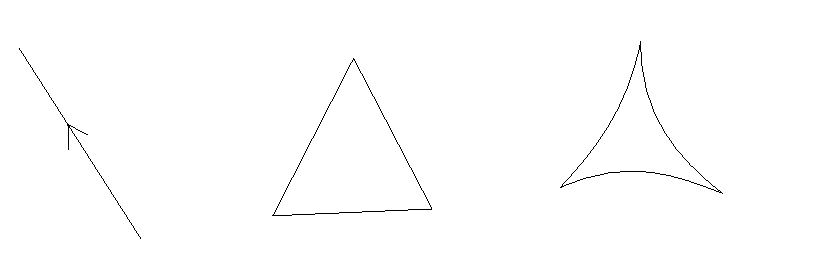
\includegraphics[width=0.8\textwidth]{img/boundary.pdf}
        \caption{Boundary Map}
        \label{fig:boundary}
    \end{figure}

    \(\sigma : \Delta^1 \to X\)

    \(\partial \sigma = \sigma(e_1) - \sigma(e_0) = c_{\sigma(e_1)}=c_{\sigma(e_0)}\), endpoint - starting point.
    
    \begin{lemma}
        \(\partial_{n+1} \circ \partial_n = 0\).

        \begin{center}
            \begin{tikzcd}
                S_{n+1} X \ar[r,"\partial_{n+1}"] \ar[rr, bend right, "0"] & S_n X \ar[r,"\partial_n"] & S_{n-1} X
            \end{tikzcd}
        \end{center}

        This is the reason for \(-\) signs.
    \end{lemma}

    Then, we have,

    \[
        \begin{matrix}
            \operatorname{im} \partial_{n+1} & \subset & \ker \partial_n & \subset & S_n X \\
            n \text{-boundaries} &  & n \text{-cycles} &  & n \text{-chains}  \\
        \end{matrix} 
    \]

    \begin{definition}
        [Singular Homology]

        \[
            H_n X = \frac{\ker \partial_n}{\operatorname{im} \partial_{n+1}} = \frac{\text{cycles}}{\text{boundaries}}
        \]
    \end{definition}

    \begin{proof}
        We prove the lemma: \(\partial_{n-1} \circ \partial_n = 0\).

        \[
            \partial_{n-1} (\partial_n \sigma)
        \]

        \[
            = \partial_{n-1} \left( \sum_{j} (-1)^{j} \sigma(t_0, \cdots , 0, \cdots , t_{n-1}) \right) 
        \]

        \[
            = \sum_{k < j} (-1)^k (-1)^j \sigma(t_0, \cdots , 0, \cdots , 0, \cdots , t_n) \, \text{\(0\) s in \(k\)'th and \(j\)'th slots}
        \]

        \[
            + \sum_{k > j} (-1)^{k-1} (-1)^j \sigma(t_0, \cdots , 0, \cdots , 0, \cdots , t_n) \, \text{\(0\) s in \(k\)'th and \(j\)'th slots}
        \]

        \[
            = 0
        \]
    \end{proof}

    \begin{remark}
        \begin{enumerate}[label=\arabic*)]
            \item \(H_n X\) is defined for any topological space \(X\) and \(n \geq 0\).
            
            \item \(X \cong Y \implies H_n X \cong H_n Y\).
            
            \item Big and Formula Construction.
            
            \item Unclear how to compute.
        \end{enumerate} 
    \end{remark}

    Answer to the question: What is \(H_n X\):

    \[
        H_{\ast} X = \left\{ H_0 X, H_1 X, H_2 X , \cdots  \right\} 
    \]

    is a graded abelian group. \(H_k X\) individually are abelian groups.

    \begin{lemma}[Lemma 1]
        \[
            H_n(pt) \cong \begin{dcases}
                \mathbb{Z}, &\text{ if } n = 0 ;\\
                0, &\text{ otherwise} .
            \end{dcases}
        \]
    \end{lemma}

    \begin{lemma}[Lemma 2]
        If \(X\) has path-components \(\{ X_\alpha \}_{\alpha \in I}\), then,

        \[
            H_n X = \bigoplus_{\alpha \in I} H_n (X_\alpha)
        \]
    \end{lemma}

    \begin{lemma}
        [Lemma 3]
        \begin{enumerate}[label=\alph*)]
            \item \( H_0 X \cong \bigoplus_{I} \mathbb{Z} = \mathbb{Z}^{\# \text{ of path component}}\)
            \item \(X\) is path-connected, then \(H_0 X \cong \mathbb{Z}\).
        \end{enumerate} 
    \end{lemma}

    Recall:

    \begin{definition}
        \(X\) is path-connected if \(\forall a,b\in X, \exists \gamma: [0,1] \to X\) such that \(\gamma(0)=a, \gamma(1)=b\) 
    \end{definition}

    \begin{definition}
        A maximal path-connected subset of \(X\) is path-component.
    \end{definition}

    \begin{corollary}
        Homology of rational numbers is isomorphic to the homology of integers:

        \[
            H_{\ast} \mathbb{Q} \cong H_{\ast} \mathbb{Z} = (\mathbb{Z}^{\infty}, 0, 0, \cdots)
        \]

        But \(\mathbb{Q} \not\cong \mathbb{Z}\).
    \end{corollary}

    \section*{Friday, 1/17/2025}
    
    Recall:

    \(H_n X = \frac{\ker (\partial_n)}{\operatorname{im} (\partial_{n+1})} = \frac{\text{cycles}}{\text{boundary}} \in \text{homology class}\).

    We are looking for two cycles that belong to the same homology class.

    So, we want cycles \(z_1 \neq z_2\) which are homologous so that \(z_1 - z_2\) is a boundary. This implies their homology classes are equal: \([z_1] = [z_2]\).

    % insert 0 cycle example

    % insert torus example

    \section*{Algebra}

    \begin{definition}
        [Chain Complex] A \underline{chain complex} \(C_\bullet\) is a sequence:
        
        \[
            C_{\ast} = \{ C_0, C_1, C_2, \cdots \}
        \]
        
        of abelian groups with \(\partial_n : C_n \to C_{n-1}\) such that \(\partial_n \circ \partial_{n+1} = 0\).

        It looks like the following:

        \begin{center}
            \begin{tikzcd}
                \cdots \ar[r] & C_3 \ar[r, "\partial_3"] & C_2 \ar[r,"\partial_2"] & C_1 \ar[r,"\partial_1"] & C_0
            \end{tikzcd}
        \end{center}

        so that the composition of any two consecutive maps is \(0\). By conventions, \(\partial_0 = 0: C_0 \to 0\).
    \end{definition}

    Then, \(C_\bullet = \{ C_{\ast}, \partial_{\ast} \}\).

    \begin{definition}
        [Homology]

        \[
            H_n C_\bullet = \frac{\ker \partial_n}{\operatorname{im} \partial_{n+1}} = \frac{Z_n}{B_n}
        \]

        Here, \(C_n = n\)-chain.
        
        \(Z_n = \ker \partial_n, n\)-cycles
        
        \(B_n = \operatorname{im} \partial_{n+1}, n\)-boundaries.

        eg. \(S_\bullet X = \{ S_{\ast} X, \partial_{\ast} \}\) is a singular chain complex of \(X\).
    \end{definition}

    L1:

    \[
        H_n \text{pt} = \begin{dcases}
            \mathbb{Z}, &\text{ if } n=0 ;\\
            0, &\text{ otherwise} .
        \end{dcases}
    \]

    \[
        H_{\ast} (\text{pt}) = \{ \mathbb{Z},0,0,\cdots \}
    \]

    \begin{proof}
        \(\forall n, \exists ! \sigma_n : \Delta^n \to \text{pt}\).

        Then, \(\partial_1 \sigma_1 = \sigma_1 \circ \delta_0 - \sigma_1 \circ \delta_1\).

        \(\delta_0(t_0) = (0,t_0), \delta_1(t_0) = (t_0, 1)\).

        Thus, \(\partial_1 \sigma_1 = \sigma_1 \circ \delta_0 - \sigma_1 \circ \delta_1=(1-1)\sigma_0 = 0\)
        
        \(\partial_2 \sigma_2 = \sigma_2 \circ \delta_0 - \sigma_2 \circ \delta_1 + \sigma_2 \circ \delta_2 = (1-1+1)\sigma_1 = \sigma_1\).

        \(\partial_n \sigma_n = \begin{dcases}
            0, &\text{ if } n \text{ odd} ;\\
            1, &\text{ if } n \text{ even}.
        \end{dcases}\) 

        \(S_{\ast} X:\)
        
        \begin{center}
            \begin{tikzcd}
                & & \ar[r] & \mathbb{Z}\sigma_2 \ar[r] & \mathbb{Z}\sigma_1 \ar[r] & \mathbb{Z}\sigma_0 \\

                & & & \sigma_2 \ar[r,mapsto] & \sigma_1 \ar[r,mapsto] & 0 \\
                \cong & \ar[r,"1"] & \mathbb{Z} \ar[r,"0"] & \mathbb{Z} \ar[r,"1"] & \mathbb{Z} \ar[r,"0"] & \mathbb{Z}
            \end{tikzcd}
        \end{center}

        \(H_0 \text{pt} = \mathbb{Z} / 00 = \mathbb{Z}\).

        \(H_1 \text{pt} = \mathbb{Z} / \mathbb{Z} = 0\) 

        \(H_2 \text{pt} = 0 / 0 = 0\).
    \end{proof}

    L2: If \(\{ X_\alpha \}_{\alpha \in I}\) are path components of \(X\) then,

    \[
        H_n X = \bigoplus_{I} H_n X_\alpha
    \]

    \begin{proof}
        \(\sigma: \Delta^n \to X \overset{\Delta^n \text{p.c.}}{\implies} \sigma(\Delta^n)\) p.c.

        \(\implies \exists ! \alpha\) such that \(\sigma(\Delta^n) \subset X_\alpha\).

        Also \((\sigma \circ \delta_j)(\Delta^{n-1}) \subset X_\alpha\)
        
        \(S_{\ast} X = \bigoplus_{I} S_{\ast} X_\alpha\) 
    \end{proof}

    Augmentation

    \(\varepsilon : S_0 X \to \mathbb{Z}\)

    \(\varepsilon (\sum_{i} n_i \sigma_i) \coloneqq \sum_{i} n_{i}\)
    
    \(\varepsilon  \circ \partial_1 (\sigma) = \varepsilon  (\sigma \circ \delta_0 - \sigma \circ \delta_1) = 1-1 = 0\)

    Thus \(\operatorname{im} \partial_1 \subset \ker \mathscr{E}\)

    Thus, \(\exists \overline{\varepsilon}: H_0 X \to \mathbb{Z}\)

    \(\overline{\varepsilon} \left[\sum_{i} n_i \sigma_i\right] = \varepsilon \left( \sum_{i} n_i \sigma_i \right) = \sum_{i} n_i \). 

    L3:

    \begin{enumerate}[label=\arabic*)]
        \item If \(X\) is path connected then,
        
        \[
            \overline{\varepsilon}: H_0 X \xrightarrow{\cong}\mathbb{Z}
        \]

        \item If \(\{ X_\alpha \}_{\alpha \in I}\) are path components of \(X\) then,
        
        \[
            H_0 X = \bigoplus_{I} H_0 X_\alpha = \mathbb{Z}^{\text{\# of p.c. of } X} 
        \]
    \end{enumerate}
    
    \begin{proof}
        \begin{enumerate}[label=\arabic*)]
            \item Need to show \(\ker \varepsilon \subset \operatorname{im} \partial_1\).
            
            Choose base point \(x_0 \in X\).

            Suppose \(\varepsilon \left( \sum_{i} n_i \sigma_i \right) = 0\).

            Choose path \(\gamma_i: \Delta^1 \to X\) such that \(\gamma_i(\underline{e}_1) = \sigma_i(\underline{e}_0), \gamma_0(e_0) = x_0\).
            
            \(\partial_1 \left( \sum_{i} n_i \gamma_i \right) = \sum_{i} n_i \sigma_i - \sum_{i} n_i \text{cons}_{X_0} = \sum_{i} n_i \sigma_i \) 
        \end{enumerate} 
    \end{proof}

    \section*{\(\Delta\)-complex (p.102-104 of Hatcher)}

    eg torus

    \begin{center}
        \begin{tikzpicture}
            \draw[->] (0,0) -- (2,0);
        \end{tikzpicture}
    \end{center}

    % insert torus picture

    \(1 =\) \# of vertices
    
    \(3 =\) \# of edges

    \(2 =\) \# of faces

    \(\Delta_2 T \to \Delta_1 T \to \Delta_0 T\) 

    \(\cong \mathbb{Z}^2 \to \mathbb{Z}^3 \to \mathbb{Z}^1\) 

    \section*{Wednesday, 1/22/2025}
    
    \begin{definition}
        [Simplex] Let \(v_0, \cdots , v_n \in \mathbb{R}^n\).

        \[
            [v_0, \cdots , v_n] = \left\{ \sum_{i} t_i v_i \mid \sum_{i} t_i = 1, 1 \leq t_i \leq 0 \right\}
        \]

        If \(v_0 - v_1, \cdots , v_0 - v_n\) are linearily independent, then \([v_0, \cdots , v_n]\) is a \underline{geometric} \underline{\(n\)-simplex}.
    \end{definition}

    If vertices are ordered,

    \[
        \sigma_{[v_0, \cdots , v_n]} : \Delta^n \to [v_0, \cdots , v_n]
    \]

    \[
        \sum_{i} t_i e_i \mapsto \sum_{i} t_i v_i
    \]

    Note that,

    \[
        \delta_n \sigma_{[v_0, \cdots , v_n]} \equiv  \sum_{j} (-1)^j \sigma_{[v_0, \cdots , \widehat{v_j}, \cdots , v_n]}
    \]

    \(\Delta^n\) breaks up into boundary and interior.

    \[
        \Delta^n = \partial \Delta^n \cup \mathring{\Delta^n}
    \]

    \[
        \partial \Delta^n = \left\{ \sum_{i} t_i e_i \mid \text{some } t_i = 0 \right\} 
    \]

    \[
        \mathring{\Delta^n} = \left\{ \sum_{i} t_i e_i \mid t_i\neq 0 \text{ for all } i \right\} 
    \]

    \begin{definition}
        A \(\Delta\)-complex is a space \(X\) with:

        \[
            \left\{ \sigma_\alpha : \Delta^n \to X \right\} \, \text{simplices} 
        \]

        such that:

        \begin{enumerate}[label=\roman*)]
            \item \(\eval{\sigma_\alpha}_{\mathring{\Delta^n}}\) is injective.
            
            \(\forall x\in X, \exists !\) s.t. \(x\in \sigma_\alpha(\mathring{\Delta^n})\). Images of interiors partition \(X\).

            \item \(\forall \alpha, \forall j, \exists \beta\) such that:
            
            \[
                \sigma_\alpha \circ \delta_j = \sigma_\beta
            \]

            Faces of simplices are simplices.

            \item \(A \subset X\) open \(\iff \forall \sigma_\alpha, \sigma_\alpha ^{-1} A\) is open in \(\Delta^n\). ``Weak Topolofy''.
        \end{enumerate} 


    \end{definition}

    Hatcher says, one way to look at this is by taking a quotient of a disjoint union. We can consider:

    \[
        \frac{\Delta^0 \sqcup \Delta^1 \sqcup \Delta^1 \sqcup \Delta^1 \sqcup \Delta^2 \sqcup \Delta^2}{\sim}
    \]

    \begin{definition}
        [Simplicial Chain Complex] \(\Delta_n X =\) free abelian group on \(n\)-simplices:

        \[
            \Delta_{n+1} X \xrightarrow{\partial_{n+1}} \Delta_n X \to \Delta_{n-1} X \to 
        \]

        Subcompplex \(\Delta_{\ast} X \subset S_{\ast} X\) 

        \begin{center}
            \begin{tikzcd}
                \Delta_n X \ar[r,"\partial"] \ar[d, hook] & \Delta_{n-1} X \ar[d, hook] \\ S_n X \ar[r,"\partial"] & S_{n-1} X
            \end{tikzcd}
        \end{center}

        The diagram commutes.

        Simplicial Homology:

        \[
            H_{\ast} ^\Delta X \coloneqq H_{\ast} (\Delta_{\ast} X)
        \]

        \[
            H_{\ast}^\Delta X \xrightarrow{\cong} H_{\ast} X
        \]
        
    \end{definition}

    Consider the \(2\)-torus with ``ordered'' vertices:

    % insert picture

    % insert picture

    \[
        \partial U = b-c+a
    \]

    \[
        \partial L = a-c+b
    \]

    \[
        \partial a = 0v, \partial b = 0v, \partial c = 0v
    \]

    \[
        \Delta_2 T \to \Delta_1 T \to \Delta_0 T \to 0
    \]

    Then, \(\Delta_2 T\) has basis \(\mathbb{Z} U \oplus \mathbb{Z} L\)

    \(\Delta_1 T\) has basis \(\mathbb{Z} a \oplus \mathbb{Z} b \oplus \mathbb{Z} c\)
    
    \(\Delta_0 T\) has basis \(\mathbb{Z}v\)

    Now, \(H_0^\Delta T = \frac{\mathbb{Z} v}{0} \cong \mathbb{Z}\) 

    \(H_2^\Delta T = \frac{\mathbb{Z}(U-L)}{0}\cong \mathbb{Z}\).

    We only have \(U-L\) since \(\partial(n_1 U + n_2 L) = 0 \implies n_1(b-c+a) + n_2(a-c+b) = 0 \implies n_1 = -n_2\)

    \(H_1^\Delta T = \frac{\mathbb{Z}(a,b,c)}{\mathbb{Z}(a-c+b)} = \frac{\mathbb{Z}(a,b,a-c+b)}{\mathbb{Z}(a-c+b)} \cong \mathbb{Z}^2\).

    We can have a basis for homology since they are free abelian.

    Basis for \(H_0^\Delta T\) is \([v]\)
    
    Basis for \(H_1^\Delta T\) is \([a],[b]\).
    
    Basis of \(H_2^\Delta T\) is \([U-L]\).

    Matrix POV on \(H_{\ast}^\Delta T\)

    \[
        \Delta_\cdot \cong \mathbb{Z}^2 \xrightarrow{\begin{bmatrix}
            1 & 1 \\
            1 & 1 \\
            -1 & -1
        \end{bmatrix} } \mathbb{Z}^3 \xrightarrow{\begin{bmatrix}
            0 & 0 & 0
        \end{bmatrix}} \mathbb{Z}
    \]

    Integral row and column operations:

    \begin{itemize}
        \item Switch two rows (or columns)
        \item Add multiples of a row (or column) to another row (or column)
        \item Multiply row (or column) by \(\pm 1\) 
    \end{itemize} 

    These correspond to basis changes in the domain and codomain.

    If matries \(A\) and \(B\) are equivalent \((A \sim B)\) it implies:

    \[
        \ker A \cong \ker B
    \]

    \[
        \operatorname{coker}  A \cong \operatorname{coker} B
    \]

    Every integral matrix is equivalent to:

    \[
        \begin{bmatrix}
            d_1 &  &  &  \\
             & d_2 &  &  \\
             &  & \ddots &  \\
             &  &  & d_n \\
        \end{bmatrix} 
    \]

    With \(d_1 \mid d_2 \mid d_3 \mid \cdots\) 

    It is a smith normal form.

    We have:

    \[
        \begin{bmatrix}
            1 & 1 \\
            1 & 1 \\
            -1 & -1 \\
        \end{bmatrix} \sim \begin{bmatrix}
            1 & 0 \\
            1 & 0 \\
            -1 & 0 \\
        \end{bmatrix} \sim \begin{bmatrix}
            1 & 0 \\
            0 & 0 \\
            0 & 0 \\
        \end{bmatrix} 
    \]

    This is \(\partial_2\).

    \(H_2^\Delta T \cong \mathbb{Z}\) 

    \(\operatorname{im} \partial_2 \cong \mathbb{Z}\) and summand of \(\Delta_1 T\)

    \(H_1^\Delta T \cong \frac{\mathbb{Z}^3}{\mathbb{Z} \times 0 \times 0} \cong \mathbb{Z}^2\) 

    Exercise: compute kernel and cokernel of: \(\begin{bmatrix}
        9 & 3 \\
        4 & 2 \\
    \end{bmatrix} \) 

    \(\begin{bmatrix}
        9 & 3 \\
        4 & 2 \\
    \end{bmatrix} \sim \begin{bmatrix}
        5 & 1 \\
        4 & 2 \\
    \end{bmatrix} \sim \begin{bmatrix}
        5 & 1 \\
        -1 & 1 \\
    \end{bmatrix} \sim \begin{bmatrix}
        6 & 0 \\
        -1 & 1 \\
    \end{bmatrix} \sim \begin{bmatrix}
        6 & 0 \\
        0 & 1 \\
    \end{bmatrix} \sim \begin{bmatrix}
        1 & 0 \\
        0 & 6 \\
    \end{bmatrix} \) 

    Thus, \(\ker = 0, \operatorname{coker} = \mathbb{Z} / 6\mathbb{Z}\).

    \section*{Friday, 1/24/2025}
    
    Goal: if there is continuous \(f: X \to Y\) then we have homomorphism \(f_{\ast} : H_{\ast} X \to H_{\ast} Y\).
    
    We think of them in terms of Category Theory.

    Setup:

    Category \(\mathcal{C}\).

    Collection of objects \(\operatorname{Ob} \mathcal{C}\).

    \(\forall X, Y \in \operatorname{Ob} \mathcal{C}\) we have a collection of morphisms \(\mathcal{C}(X,Y)\).

    \(\forall X,Y,Z \in \operatorname{Ob} \mathcal{C}\) we have composition law:

    \[
        \mathcal{C}(X,Y) \times \mathcal{C}(Y,Z) \to \mathcal{C}(X,Z)
    \]

    \[
        (g,f) \mapsto f \circ g
    \]

    Also, \(\forall X\in \operatorname{Ob} \mathcal{C}, \exists \operatorname{id}_{X} \in \mathcal{C}(X,X)\).

    We also have associative law:

    \[
        (f \circ g) \circ h = f \circ (g \circ h)
    \]

    \(\forall f\in \mathcal{C}(X,Y), f = \operatorname{id}_{Y} \circ f = f \circ \operatorname{id}_{X}\).

    For \(f\in \mathcal{C}(X,Y)\) we can also write it as \(f: X \to Y\) or \(X \xrightarrow{f} Y\).

    We sometimes call them `arrows' instead of `morphisms' to avoid thinking of them as functions.

    \begin{center}
        \begin{tikzcd}
            X \ar[r,"g"] \ar[rr, bend right, "f\circ g"'] & Y \ar[r,"f"] & Z
        \end{tikzcd}
    \end{center}

    \begin{definition}
        \(f: X \to Y\) is an \underline{isomorphism} if \(\exists g: Y \to X\) such that:

        \[
            f \circ g = \operatorname{id}_{Y}, g \circ f = \operatorname{id}_{X} 
        \]

        We write it as \(X \cong Y\) and say \(X\) and \(Y\) are \underline{isomorphic}.
    \end{definition}

    Example of Categories:

    \(\operatorname{Set}\) is (sets, functions).

    \(\operatorname{Top}\) is (topological spaces, continuous functions)

    \(\operatorname{Ab}\) is (abelian groups, homomorphisms)

    Morphisms need not be functions!!

    A group can be viewed as a category with one object. Elements of the group is the set of morphisms, and all morphisms are invertible.

    Suppose \(G = \{ 1,T \}\) of order \(2\). Then, we have:

    \begin{center}
        \begin{tikzcd}
            T \ar[loop left, "T"] \ar[loop right, "\operatorname{id}"]
        \end{tikzcd}
    \end{center}

    Where \(T \circ T = \operatorname{id}\) 

    We let \(\operatorname{Ch}\) be the category of \underline{chain complexes}.

    The objects will be chain complexes. What are the morphisms?

    Recall that Chain complexes are \(C_\bullet = (C_{\ast} , \partial_{\ast})\) where:

    \begin{center}
        \begin{tikzcd}
            \, \ar[r] & C_{n+1} \ar[r,"\partial_{n+1}"] & C_n \ar[r,"\partial_n"] & C_{n-1} \ar[r] & \,
        \end{tikzcd}
    \end{center}

    Where \(\partial_{n+1} \circ \partial_n = 0\).
    
    Morphisms are given by \underline{chain maps}.

    \begin{definition}
        [Chain map] \(f_\bullet: C_\bullet \to C_\bullet^{\prime}\) is a sequence of homomorphisms \(f_n : C_n \to C_n^{\prime}\) such that:

        \[
            f_{n-1} \circ \partial_n = \partial_n^{\prime} \circ f_n
        \]

        For all \(n\).
    \end{definition}

    We have the following commutative diagram:

    \begin{center}
        \begin{tikzcd}
            \, \ar[r] & C_{n+1} \ar[d] \ar[r] & C_n \ar[d] \ar[r] & C_{n-1} \ar[d] \ar[r] & \, \\
            \, \ar[r] & C_{n+1}' \ar[r] & C_n' \ar[r] & C_{n-1}' \ar[r] & \,
        \end{tikzcd}
    \end{center}

    For example, if we have \(f: X \to Y\) we have the chain map:

    \[
        f_\# = S_\bullet f : S_\bullet X \to S_\bullet Y
    \]

    Given by:

    \[
        (S_{\bullet} f) \left( \sum_{i} n_i \sigma_i \right) \coloneqq \sum_{i} n_i (f \circ \sigma_i)
    \]

    % insert picture

    This gives us:

    \begin{center}
        \begin{tikzcd}
            S_n X \ar[r,"\partial_n"] \ar[d, "S_n f"] & S_{n-1} X \ar[d] \\ S_n Y \ar[r,"\partial_n"] & S_{n-1} Y
        \end{tikzcd}
    \end{center}

    \begin{lemma}
        A chain map \(f_\bullet: C_\bullet \to C_\bullet^{\prime} \) induces \(f_{\ast} = H_n(f_\bullet) : H_n C_\bullet \to H_n C_\bullet^{\prime}\) given by \([x] \mapsto [f_n x]\)  
    \end{lemma}

    \begin{remark}
        elements in \(\frac{\ker \partial_n}{\operatorname{im} \partial_{n+1}}\) can be \([x]\) [equivalence classes] or \(x + \operatorname{im} \partial_{n+1}\) [cosets]. We use equivalence classes:

        \(x \sim x^{\prime} \iff x - x^{\prime} \in \operatorname{im} \partial\) 
    \end{remark}

    \begin{proof}
        \(f_n(\text{cycles}) \subset \text{cycles}\).
        
        \(f_n(\text{boundaries}) \subset \text{boundaries}\).
        
        Recall that cycle is \(\ker \partial_n\).

        Consider a cycle \(X\). Then, \(\partial X = 0 \implies f(\partial x) = 0 \implies \partial ^{\prime} f(x) = 0 \implies f(x) \in \ker \partial ^{\prime}\).

        Boundary is \(\operatorname{im} \partial_{n+1}\).

        \(f(\partial y) = \partial ^{\prime} f(y) \in \operatorname{im} \partial_{n+1}^{\prime}\).

        Thus we have:
        
        \[
            \ker \partial_n \to \ker \partial_n^{\prime} \to \frac{\ker \partial_n^{\prime}}{\operatorname{im} \partial_{n+1}^{\prime}}
        \]

        This induces,

        \[
            \frac{\ker \partial_n}{\operatorname{im} \partial_{n+1}} \to \frac{\ker \partial_n^{\prime}}{\operatorname{im} \partial_{n+1}^{\prime}}
        \]

    \end{proof}

    Now we move on to functors. Functors are an analogy of functions on Categories.

    Consider two categories \(\mathcal{C}\) and \(\mathcal{D}\). We want to define a functor between them.

    \begin{definition}
        A functor \(F: \mathcal{C} \to \mathcal{D}\) will be an `assignment' of objects and morphisms.
        
        We have \(F: \operatorname{Ob} \mathcal{C} \to \operatorname{Ob} \mathcal{D}\).
        
        \(\forall X,Y \in \operatorname{Ob} \mathcal{C}\) we have:

        \[
            F: \mathcal{C}(X,Y) \to \mathcal{D}(F(X),F(Y))
        \]

        Then, \(F(f \circ g) = F(f) \circ F(g)\).

        \(F(\operatorname{id}_{X}) = \operatorname{id}_{F(X)}\) 
    \end{definition}

    So we can \(F\) a whole category:

    \[
        X \xrightarrow{f} Y
    \]

    \[
        F(X) \xrightarrow{F(f)} F(Y)
    \]

    We have the \underline{singular} functor taking topological spaces to chain complexes. We also have functor taking chain complexes to abelian groups.

    \[
        \operatorname{Top} \xrightarrow{S_\bullet} \operatorname{Ch} \xrightarrow{H_n} \operatorname{Ab} 
    \]

    We also have forgetful functor which forgets:

    \[
        \operatorname{Ab} \to \operatorname{Set} 
    \]

    \[
        \operatorname{Ab} \to \operatorname{Group} 
    \]

    We have the category \(\operatorname{Gr}\) of graded abelian groups.

    \(\operatorname{Gr}\) has objects \(A_{\ast} = \{ A_0, A_1, A_2, \cdots \} \) set of abelian groups, and morphisms \(A_{\ast} \xrightarrow{f_0} B_{\ast}\).
    
    Then we can write:

    \begin{center}
        \begin{tikzcd}
            \operatorname{Top} \ar[r,"S_\bullet"] \ar[rrr, bend right, "H_n"] & \operatorname{Ch} \ar[r,"H_{\ast}"] & \operatorname{Gr} \ar[r,"H_n"] & \operatorname{Ab}
        \end{tikzcd}
    \end{center}

    \begin{lemma}
        Consider a functor \(F: \mathcal{C} \to \mathcal{D}\). Then, \(X \cong Y \implies F(X) \cong F(Y)\).
    \end{lemma}

    Corollary: \(X \cong Y\) (homeomorphic) implies \(H_n X \cong H_n Y\) 

    \begin{proof}
        \(X\cong Y\) implies we have \(f,g\) so that \(f(X)=Y, g(Y) = X\) so that \(f \circ g = \operatorname{id}_{Y}, g \circ f = \operatorname{id}_{X}\).
        
        Then, \(F(f) \circ F(g) = F(f \circ g) = F(\operatorname{id}_{Y}) = \operatorname{id}_{F(Y)}\). Similar for \(g \circ f\). So, \(F(f)\) and \(F(g)\) are isomorphisms and thus \(F(X)\) and \(F(Y)\) are isomorphic. 
    \end{proof}

    \section*{Monday, 1/27/2025}
    
    \section*{Homotopy Invariance of Homology}

    \begin{definition}
        [Homotopy] \(H: X \times I \to Y\, I = [0,1]\).

        Homotpy is a `path' of map \(H_t: X \to Y\) where \(t\in [0,1]\) is `time'. \(H_t(x) = H(x,t)\).
    \end{definition}

    % insert picture

    \begin{definition}
        \(f,g : X \to Y\) are \underline{homotopic} if there exists \(H: X \times I \to Y\) such that \(H_0 = f, H_1 = g\).
    \end{definition}

    If they're homotopic we write \(f\simeq g\).

    \begin{theorem}
        [Homotopy Theorem]

        \[
            f \simeq g \implies H_{\ast} f = H_{\ast} g: H_{\ast} X \to H_{\ast} Y
        \]

        \[
            f_{\ast} = g_{\ast} 
        \]
    \end{theorem}

    Fact/Exercise: \(\simeq\) is a equivalence relation on \(\operatorname{TOP}(X,Y)\) 

    \([X,Y] = \operatorname{TOP}(X,Y) / \simeq =\) homotopy classes of map \(X \to Y\).

    Suppose for \(X,Y\), \(X \xleftrightarrow[g]{f} Y\) we have \(f \circ g \simeq \operatorname{id}_X,X \cong H_{\ast} Y\).
    
    For example, \(\mathbb{R}^2 - 0 \simeq S^1\). by \(x \xmapsto{f} \frac{x}{\vert x \vert}\) and \(g = \text{inclusion}\).

    Straight line homotopy \(tx + (1-t) \frac{x}{\vert x \vert}\)

    \begin{definition}
        \(X\) \underline{contractible} if \(X \simeq pt\).

        eg \(\mathbb{R}^2 \simeq \ast\) 
    \end{definition}

    % insert picture

    \begin{definition}
        Homotopy Category \(\operatorname{hTOP}\).

        \underline{Objects}: Topological Spaces [\underline{NOT} HOMOTOPY EQUIVALENCE CLASSES]

        \underline{Morphisms}: \(\operatorname{hTOP}(X,Y) = [X,Y]\). [These are Equivalence Classes]
        
        \underline{Exercise}: Composition is well defined. So, \(f \simeq f^{\prime} , g \simeq g^{\prime} \implies f \circ g \simeq f
        \circ g^{\prime}\). Then, \([f] \circ [g] \coloneqq [f \circ g]\) 
    \end{definition}

    \subsection*{Isomorphisms in hTOP}

    \(X,Y\) Isomorphic in \(\operatorname{hTOP} \iff X \simeq Y\) [homotopy equivalence].

    So, homotopy theorem says homology factors through homotopy:

    \begin{center}
        \begin{tikzcd}
            \operatorname{hTop}\ar[r,"H_\ast"] & \operatorname{Gr} \\ \operatorname{TOP} \ar[u] \ar[ur, "H_\ast"']
        \end{tikzcd}
    \end{center}

    Thus, \(X \simeq Y \iff H_{\ast} X \implies H_{\ast} Y\) is really just a consequence of homotopy theorem.

    \begin{definition}
        \(A \subset X\), then \(A \) is a \underline{deformation retract} of \(X\) `if we can deform all of \(X\) into \(A\)'. Formally,

        if \(\exists H: X \times I \to X\) such that:
        
        \(\forall x\in X, H(x,0)=x, H(x,1)\in A\) and \(H(a,1)=a \forall a\in A\).

        Suppose \(A \simeq X\), \(A \xhookrightarrow{i} X, A \xleftarrow{H_1} X\).

        \(\operatorname{id}_{A} = H_1 \circ i, \operatorname{id}_{X} \underset{H}{\simeq} i \circ H_1\)

        eg M\"obius strip \((X)\) is homotopy equivalent to the cure circle \(A\).

        % insert picture

        \begin{definition}
            \(X \subset \mathbb{R}^n\) is start shaped at \(p_0 \in X\) if \(\forall p\in X, \overline{pp_0} \subset X\).
        \end{definition}

        % insert picture

        convex \(\implies\) star-shaped \(\implies\) contractable (by the straight line homotopy)

        We can take \((1-t)p_0 + ^{\top}  = H(p,t)\).

        eg the \(n\)-simplex \(\Delta^n\) and the prism \(\Delta^n \times I\) are star-shaped.

    \end{definition}

    \begin{theorem}
        \(X\) start shaped \(\implies H_{\ast} (X) = \mathbb{Z}\) or \(0\).
    \end{theorem}

    \begin{corollary}
        \(H_{\ast} (\Delta^n) \cong H_{\ast} (pt)\)

        \(H_{\ast} (\Delta^n \times I) \cong H_{\ast} (p t)\).
    \end{corollary}

    \begin{proof}
        Wlog \(\sigma : \Delta^n \to X\).

        Syspension \(s \sigma : \Delta^{n=1} \to X\):

        \[
            s \sigma(t_0, \cdots , t_{n+1}) = \begin{dcases}
                (1-t_0) \sigma \left( \frac{t_1}{1-t_0}, \cdots , \frac{t_{n+1}}{1-t_0} \right), &\text{ if }  t_0 \neq 1 ;\\
                0, &\text{ if } t_0 = 1 .
            \end{dcases}
        \]

        % insert picture

        We will show that if \(z\) is a \(n\)-cycle with \(n > 0\) then \(z = \partial (s z) \implies z\) is a boundary.

        Define: \(0\)th face of \(s \sigma\) is \(\sigma\).

        \((s \sigma) \circ \delta_0 = \sigma\)

        \((s \sigma) \circ \delta_{j+1} = s(\sigma \circ \delta_j) \implies s \partial + \partial s = \operatorname{id}_{S_n X} \, \forall n > 0\).

        Thus if \(z \in S_n X\) then ,

        \(s \partial z + \partial s z = z \implies \partial(sz) = z \implies z\) is a boundary.
    \end{proof}

    \subsection*{Algebra}

    \begin{definition}
        Chain map \(f_\bullet, g_\bullet: C_\bullet \to C_{\bullet}^{\prime}\) are \underline{chian} \underline{homotopic} if \(\exists\) homomorphisms \(h_n : C_n \to C_{n+1}
    ^{\prime}\)  `degree one' such that:

    \[
        \partial ^{\prime} h + h_{n-1} \partial _n = f_n - g_n
    \]

    \begin{center}
        \begin{tikzcd}
            C_{n+1} \ar[r] & C_n \ar[ld,"h"] \ar[d, "f-g"] \ar[r] & C_{n-1} \ar[ld, "h"] \\ C_{n+1}^\prime \ar[r] & C_n^\prime \ar[r] & C_{n-1}^\prime
        \end{tikzcd}
    \end{center}
    \end{definition}

    \section*{Wednesday, 1/29/2025}
    
    We write it as \(f_\bullet \underset{h}{\simeq} g\) if \(\partial ^{\prime} _{n+1} h_n + h_{n-1} \partial_n = f_n - g_n\). Then \(f_\bullet\) and \(g_\bullet\) are chain homotopic.

    Homotopy theorem: \(f\simeq g: X \to Y \implies f_{\ast} =g_{\ast} : H_{\ast} X \to H_{\ast} Y\)

    \(\star\) Exercise: \(f_\bullet \simeq g_\bullet \implies H_n(f_\bullet) = H_n(g_\bullet): H_n(C_\bullet) \to H_n(C^{\prime}_\bullet)\).

    Hint: \((f_n - g_n)(\text{cycle}) = \in \text{boundary}\)

    \(\star\star\) \(H_n(\Delta^n \times I) = 0\) for all \(n > 0\).
    
    \(\Delta^n \times I \subset \mathbb{R}^{n+1}\)

    convex \(\implies\) star shaped.

    \underline{Homotopy}: \(\operatorname{id}_{}: X \times I \to X \times I\)

    % insert picture

    Let \(\eta_1 \simeq \eta_0: X \to X \times I\)

    \(\eta_0(x) = (x,0)\)

    \(\eta_1(x) = (x,1)\)

    What we want to show that our theorem is true in this case.

    \begin{lemma}
        \(\exists\) homomorphism \(P_n^X: S_n X \to S_{n+1} (X \times I)\), natural in \(X\), such that \(\partial P + P \partial = S(\eta_1) - S(\eta_0)\).

    \end{lemma}
    
    \begin{proof}
        Recall that \(S_n: \operatorname{TOP} \to \operatorname{Ab}, \eta_0: X \to X \times I \implies S_n(\eta_0): S_n X \to S_n X \times I \eqqcolon \eta_{0\#}\) is given by composition:

        \[
            \eta_{0\#} \left( \sum_{i} n_i \sigma_i \right) = \sum_{i} n_i (\eta_0 \circ \sigma_i)
        \]

        We prove by induction on \(n\).

        \(N_n\) by `naturality': \(X \xrightarrow{f} Y\) and we have commutative diagram:

        \begin{center}
            \begin{tikzcd}
                S_n X \ar[r] \ar[d] & S_n Y \ar[d] \\ S_{n+1} (X \times I) \ar[r] & S_{n+1}(Y \times I)
            \end{tikzcd}
        \end{center}


        \((H_n): \, \partial_{n+1} P_n^X + P_{n-1}^X \partial_n = S_n(\eta_1) - S_n(\eta_0)\).

        \(n=0\): \(0 = P_{-1}: 0 \to S_0(X \times I)\).

        \(P_0(\sigma) (t_0, t_1) = (\sigma(0),t_1)\) 

        boundary of 1 chain is subtraction of midpoint.

        \(\partial P_0(\sigma) = \eta_1 \circ \sigma - \eta_0 \circ \sigma\)
        
        Assume \(P_0^X, \cdots, P_0^X, \cdots , P_{n-1}^X\) are defined satisfying Hs and Ks.

        Let \(\iota = \iota_n = \operatorname{id}_{\Delta^n}\). Goal is to define \(P_n^{\Delta^n}(\iota) \in S_{n+1} (\Delta^n \times I)\).

        We want \(H_n\) to hold.

        So we want \(\partial P(\iota) = \eta_{1\#}\iota - \eta_{0\#} \iota - P \partial \iota\).
        
        So we basically want to know whether \(\eta_{1\#}\iota - \eta_{0\#}\iota - P \partial \iota\) is a cycle.

        We see \(\partial (\eta_{1\#}\iota - \eta_{0\#}\iota - P \delta \iota)\). Since \(\eta_{i\#}\) are chain maps they commute with \(\partial\) therefore:

        \(= \eta_{1\#} \partial \iota - \eta_{0\#} \partial \iota - \partial P \partial \iota\)
        
        \(= \eta_{1\#} \partial \iota - \eta_{0\#} \partial \iota -(\eta_{1\#} - \eta_{0\#} - P \partial)(\partial i) = 0\) 

        \(\star\star \implies\) cycles = boundaries.

        Choose \(P_n \iota\) such that:

        \(\partial P_n \iota = \eta_{1\#} - \eta_{0\#} - P \partial \iota\).

        
        Now, \((N_n)\):

        \(\sigma : \Delta^n \to X, \sigma_\#: \iota \mapsto \sigma\)

        \begin{center}
            \begin{tikzcd}
                S_n\Delta^n \ar[d,"P"] \ar[r,"\sigma\#"] & S_n X\ar[d] \\ S_{n+1}(\Delta^{n}\times I) \ar[r,"(\sigma\times id)_{\#}"] & S_{n+1}(X\times I)
            \end{tikzcd}
        \end{center}

        Define \(P \sigma = (\sigma \times \operatorname{id}_{})_\# P \iota\) 

    \end{proof}
    
    % insert picture

    \begin{theorem}
        [Homotopy Theorem] \(f\simeq g: X \to Y \implies f_{\ast} = g_{\ast} : H_{\ast} X \to H_{\ast} Y\).
    \end{theorem}

    \begin{proof}
        \(H: X \times I \to Y\). We want \(h_n: S_n X \to S_{n+1} Y\) such that:
        
        \[
            \partial h + h \partial = H_{1\#} - H_{0\#}
        \]

        Note: \(H_i = H \circ \eta_i\)

        We define \(h_n \sigma \coloneqq H_\# (P_n \sigma)\) 

        \((\partial h + h \partial)\sigma = \partial H_\# P \sigma + H_\# P_n \partial \sigma = H_\# (\partial P \sigma + P \partial \sigma) = H_\# (\eta_{1\#} - \eta_{0\#})\sigma = H_{1\#}\sigma - H_{0\#}\sigma\) 
    \end{proof}

    \section*{Friday, 1/31/2025}
    
    Exact sequences

    Long Exact Sequences (LES)

    Short Exact Sequences (SES)

    Mayer-Vietoris Exact Sequences (MVES)

    \(A \xrightarrow{\alpha} B \xrightarrow{\beta} C\) is \underline{exact} if \(\operatorname{im} \alpha = \ker \beta\) 
    
    \(\iff \operatorname{im} \alpha \subset \ker \beta\) and \(\operatorname{im} \alpha \supset \ker \beta\)

    Note that \(\operatorname{im} \alpha \subset \ker \beta \iff \beta \circ \alpha =0\)

    A sequence \(C_n \to C_{n-1} \to \cdots C_1 \to 0\) if it is exact at \(C_{n-1}, \cdots , C_1\).

    Sequence,

    \[
        \cdots \to C_{n+1} \to C_n \to C_{n-1} \to \cdots 
    \]

    is exact if it is exact at \(C_i\) for all \(i\). LES.

    \(\cdots \to C_{n+1} \to C_n \to C_{n-1} \to \cdots\) is exact \(\iff C_\bullet\) is a chain complex and \(H_{\ast} C_\bullet = 0\).

    \(0 \to A \xrightarrow{\alpha} B\) is exact \(\iff \ker \alpha = 0 \iff \alpha\) is injective / 1-1.
    
    Dual: \( A \xrightarrow{\alpha} B \to 0\) is exact \(\iff \operatorname{im} \alpha = B \iff \alpha\) is surjective / onto.

    \(0 \to A \xrightarrow{\alpha} B \to 0\) exact \(\iff \alpha\) is 1-1 and onto \(\iff \alpha\) is an isomorphism.

    If \(A \hookrightarrow B\) then \(0 \to A \to B \to B / A \to 0\) is exact.

    If \(A \xrightarrow{f} B\) then \(0 \to \ker f \to A \xrightarrow{f} B \to \operatorname{coker} f \to 0\).

    Short Exact Sequence:

    Suppose \(0 \to A \xrightarrow{\alpha} B \xrightarrow{\beta} C \to 0\)

    \(\iff \alpha\) 1-1, \(\beta\) onto, \(\operatorname{im} \alpha = \ker \beta \iff \alpha\) 1-1, \(\overline{\beta} : B / \operatorname{im} \alpha \xrightarrow{\cong} C \to 0\) 

    \begin{center}
        \begin{tikzcd}
            0 \ar[r] & A \ar[d,"\cong"] \ar[r,"\alpha"] & B\ar[d,"="] \ar[r,"\beta"] & C \ar[d,"\cong"',"(\overline{\beta})^{-1}"] \ar[r] & 0 \\
            0 \ar[r] & \alpha(A) \ar[r] & B \ar[r] & \, \ar[r] & 0
        \end{tikzcd}
    \end{center}

    Canonical Example:

    \(0 \to \mathbb{Z} / 2 \to \mathbb{Z} / 4 \to \mathbb{Z} /2 \to 0\) and \(0 \to \mathbb{Z} /2 \to \mathbb{Z} / 2 \oplus \mathbb{Z} /2 \to \mathbb{Z} /2 \to 0\).

    Spaces \(A,B \subset X\)

    \begin{center}
        \begin{tikzcd}
            A\cap B \ar[r, hook, "i"] \ar[d,hook,"j"] & A \ar[d,hook,"k"] \\ B \ar[r, hook, "\ell"] & X
        \end{tikzcd}
    \end{center}
    
    \begin{theorem}
        [Mayer-Vietoris Exact Sequence]

        If \(X = \operatorname{int} A \cup \operatorname{int} B\) [eg \(X = A\cup B, A, B\) open]

        Then \(\exists\) LES:

        \[
            \cdots \to H_n A \cap B \xrightarrow{i_{\ast} \oplus j_{\ast}} H_n A \oplus H_n B \xrightarrow{k_{\ast} - \ell_{\ast}} H_n X \xrightarrow{\partial} H_{n-1} A \cap B
        \]

        \[
            \cdots \to H_0 X \to 0
        \]
    \end{theorem}

    We need \(\partial [\alpha]\). If \(\alpha\) is a cycle in \(X\) we have,

    \[
        \alpha \underset{\text{homologous}}{\sim} \alpha_A + \alpha_B
    \]

    Meaning \(\alpha - (\alpha_A + \alpha_B)\) is a boundary.

    Furthermore, \(\partial [\alpha] = \partial [\alpha_A]\).

    Homology of a circle \(S^1\).

    Circle can be written as union of \(A = \cup\) and \( B = \cap\).

    Then \(A \simeq pt, B \simeq pt, A\cap B \simeq 2 pts\) which is \(S^0\).

    \(H_1 S^1 \xrightarrow{\partial} H_0 A \cap B \to H_0 A \oplus  H_0 B \to H_0 S^1 \to 0\) 

    \(0 \to H_1 S^1 \to \mathbb{Z}^2 \xrightarrow{\begin{bmatrix}
        1 & 1 \\
        1 & 1 \\
    \end{bmatrix}} \mathbb{Z}^2 \to H_0 S^1 \to 0\)
    
    Thus, \(H_1 S^1 = \ker \begin{bmatrix}
        1 & 1 \\
        1 & 1 \\
    \end{bmatrix} = \mathbb{Z} \begin{bmatrix}
        1 \\
        -1 \\
    \end{bmatrix} \cong \mathbb{Z}\) 

    \(H_0 S^1 = \operatorname{coker} \begin{bmatrix}
        1 & 1 \\
        1 & 1 \\
    \end{bmatrix} \cong \mathbb{Z}\).
    
    \(0 \to H_n S^1 \to 0 \to  \implies H_n S^1 = 0\).

    For \(n > 0\), the homology of \(S^n\) can be done similarly with 2 \(D^n\).

    \[
        H_i S^n \cong \begin{dcases}
            \mathbb{Z}, &\text{ if } i=0,n ;\\
            0, &\text{ otherwise} .
        \end{dcases}
    \]

    Can be proven via MVES and induction on \(n\).

    \section*{Monday, 2/3/2025}
    
    \begin{theorem}
        For \(n > 0\), we have:

        \[
            H_i S^n \cong \begin{dcases}
                \mathbb{Z}, &\text{ if } i = 0,n ;\\
                0, &\text{ otherwise} .
            \end{dcases}
        \]
    \end{theorem}

    \begin{proof}
        MVES + induction on \(n\).

        For \(n = 1\):

        Homology of a circle \(S^1\).

        Circle can be written as union of \(A = \cup\) and \( B = \cap\).
    
        Then \(A \simeq pt, B \simeq pt, A\cap B \simeq 2 pts\) which is \(S^0\).
    
        \(H_1 S^1 \xrightarrow{\partial} H_0 A \cap B \to H_0 A \oplus  H_0 B \to H_0 S^1 \to 0\) 
    
        \(0 \to H_1 S^1 \to \mathbb{Z}^2 \xrightarrow{\begin{bmatrix}
            1 & 1 \\
            1 & 1 \\
        \end{bmatrix}} \mathbb{Z}^2 \to H_0 S^1 \to 0\)
        
        Thus, \(H_1 S^1 = \ker \begin{bmatrix}
            1 & 1 \\
            1 & 1 \\
        \end{bmatrix} = \mathbb{Z} \begin{bmatrix}
            1 \\
            -1 \\
        \end{bmatrix} \cong \mathbb{Z}\) 
    
        \(H_0 S^1 = \operatorname{coker} \begin{bmatrix}
            1 & 1 \\
            1 & 1 \\
        \end{bmatrix} \cong \mathbb{Z}\).

        Thus it is indeed true for \(S_1\).

        For \(S^n\) divide Let \(N = \begin{bmatrix}
            0 \\
            \vdots \\
            1 \\
        \end{bmatrix}\) and \(S \equiv  \begin{bmatrix}
            0 \\
            \vdots \\
            -1 \\
        \end{bmatrix}\). Write \(A = S^n - \{ S \}, B = S^n - \{ B \} \).
        
        Then, \(A \simeq \{ N \}, B \simeq \{ S \}, A\cap B \simeq S^{n-1}\).

        These are deformation retracts: One way it's an inclusion, other way it is a retract.

        i. \(A \simeq N\): Use normalized straight line homotopy.

        \[
            H: A \times I \to  A, x \mapsto \frac{(1-t)x + tN}{\lVert (1-t)x + tN \rVert}
        \]

        We avoid the south pole to avoid division by \(0\).

        Same for ii.

        \(A\cap B\): We don't have north and south pole.

        Idea: project and normalize.

        Suppose \(x = (x_0, \cdots , x_n) \in A \cap B\).

        Let \(r(x)\coloneqq \frac{(x_0, \cdots , x_{n-1}, 0)}{\lVert x_0, \cdots , x_{n-1},0 \rVert }\)

        Then \(H(x,t) = \frac{(1-t) + t r(x)}{\lVert  \rVert}\).

        We're essentially going along an arc to minimize our journey throuth the sphere.

        \begin{table}[H]
            \centering
            \begin{tabular}{c|c|c|c}
                \toprule
                    \(i\) & \(H_i A \cap B\) & \(H_i A \oplus H_i B\) & \(H_i S^n\) \\
                    & \(\cong H_i(S^{n-1})\) & \(\cong H_i(pt) \oplus H_i(pt)\) & \\  
                \midrule
                    \(0\)  & \(\mathbb{Z}\)  & \(\mathbb{Z} \oplus \mathbb{Z}\) & \(\mathbb{Z}\) \\
                    \(1\)  & \(0\) & \(0\) & ? \\
                    \(\vdots\)  &  &  &  \\
                    \(n-1\)  & \(\mathbb{Z}\) & \(0\) & ? \\
                    \(n\) & \(0\) & \(0\) & ? \\
                \bottomrule
            \end{tabular}
            \caption{MVES for \(S^n\)}
        \end{table}

        All question marks should be \(0\) except for the last one since it maps to \(\mathbb{Z}\).

        Application for \(H_{\ast} S^n: S^n \simeq S^m \implies n = m\).

    \end{proof}

    \begin{definition}

        \(A \subset X\) is a retract if \(\exists\) continuous \(r: X \to A\) such that \(r(a) = a \forall a\in A\).

        \(A\) is a retract. \(r\) is a retraction.

        Thus, retract means \(r\) is a left inverse of the inclusion map \(i: A \to X\).

        By functoriality, the same thing is true once we pass to homology.

        \(r_{\ast} \circ i_{\ast} = \operatorname{id}_{H_{\ast} A} \implies  H_{\ast} X = i_{\ast} H_{\ast} A \oplus \ker r_{\ast}\).
    \end{definition}

    \begin{theorem}
        [Brouwer No Retraction Theorem] \(S^{n-1}\) is \underline{not} a retract of \(D^n\).
    \end{theorem}

    \begin{proof}
        We use contradiction. Assume \(\exists r: D^n \to S^{n-1}\) such that \(\eval{r}_{S^{n-1}}^{} = \operatorname{id}_{}\).

        \begin{center}
            \begin{tikzcd}
                S^{n-1} \ar[r,"i"] \ar[rr, bend right, "id"] & D^n \ar[r,"r"] & S^{n-1}
            \end{tikzcd}
        \end{center}

        Applying the functor \(H_n\), 

        \begin{center}
            \begin{tikzcd}
                H_n S^{n-1} \ar[r,"i_*"] \ar[rr, bend right, "id"] & H_n D^n \ar[r,"r_*"] & H_n S^{n-1}
            \end{tikzcd}
        \end{center}

        \(D^n\) is retractible. When \(n > 1\) we have \(H_{n-1} D^n = \mathbb{Z}\).

        \begin{center}
            \begin{tikzcd}
                \mathbb{Z} \ar[r] \ar[rr, bend right, "id"] & 0 \ar[r] & \mathbb{Z}
            \end{tikzcd}
        \end{center}

        Which cannot happen.

    \end{proof}

    \begin{theorem}
        [Brower Fixed Point Theorem] Every \(f: D^n \to D^n\) has a fixed point.
    \end{theorem}

    \begin{proof}
        Assume there doesn't exist a fixed point.

        Then we can construct a retraction map \(r: D^n \to S^n\) by drawing a line from \(f(x)\) to \(x\) and intersecting it with boundary.
    \end{proof}

    \subsection*{Relative Homology}

    Goal: exact of a pair \(A \subset X\).

    \[
        \cdots \to H_n A \to H_n X \to H_n(X,A) \xrightarrow{\partial} H_{n-1} \to \cdots 
    \]

    \(H_n(X,A)\): ``relative homology''. We extract `relative cycles'.

    Chain is a formal linear combination. We require the boundary be in \(A\).

    \begin{definition}
        [Category of Pairs] \(\operatorname{Top}^2\).

        Objects: \((X,A)\) where \(A \subset X\) open.

        Morphism: \((X,A) \to (Y,B)\) is a continuous map \(f: X \to Y\) so that \(f(A) \subset B\).
    \end{definition}

    We have a functor \(H_n: \operatorname{Top}^2 \to \operatorname{Ab}\).

    \begin{center}
        \begin{tikzcd}
            S_n A \ar[d,hook] \ar[r,"\partial"] & S_{n-1} A \ar[d,hook] \\ S_n X \ar[r,"\partial"] & S_{n-1} X
        \end{tikzcd}
    \end{center}

    This means we have \(S_n X / S_n A \xrightarrow{\overline{\partial }} S_{n-1} X / S_{n-1} A\) 

    Relative Chain complex:

    \[
        S_\bullet(X,A) = \left\{ \frac{S_{\ast} X}{S_{\ast} A}, \overline{\partial } \right\} 
    \]

    \section*{Wednesday, 2/5/2025}
    
    Suppose we have a Mayer-Vietoris Exact sequence.

    \[
        \cdots \to H_n (A \cap B) \xrightarrow{H_n(i) \oplus H_n(j)} H_n(A) \oplus H_n(B) \to \underline{H_n X} \to H_{n-1} (A\cap B) \to \cdots  
    \]

    Then we have the following short exact sequence:

    \[
        0 \to \operatorname{coker} (H_n i \oplus H_n j) \to H_n X \to \ker (H_n i \oplus H_n j) \to 0
    \]

    Then, \(H_n X\) is determined upto an extension.

    If \(\operatorname{coker} = \mathbb{Z} / 2, \ker = \mathbb{Z} / 2\) then \(H_n X\) can be \(\mathbb{Z} / 4\) or \(\mathbb{Z} / 2 \oplus \mathbb{Z} / 2\).

    If all of them are free [so maps are matrix maps] then we can use smith normal form.

    This gives us: \(H_n S^n \cong H_{n-1} S^{n-1}\).

    \begin{remark}
        Generator of \(H_n S^n\) is represented by:

        \[
            \Delta^n \to \Delta^n / \partial \Delta^n \cong S^n
        \]

        or,

        \[
            \partial_{n+1} ( \Delta^{n+1} \to \Delta^{n+1})
        \]

        aka sum of top simplicies of \(\partial \Delta^n\).
    \end{remark}

    \subsection*{Relative Homology}

    Consider the pair \((X,A)\) with \(A \subset X\).

    \begin{definition}
        [Singular Relative Chain Complex]

        \[
            S_\bullet(X,A) = \left\{ S_{\ast} (X,A), \overline{\partial} \right\} 
        \]

        \[
            \cdots \to S_{n+1} (X,A) \xrightarrow{\overline{\partial}_{n+1}} S_n(X,A) \xrightarrow{\overline{\partial}_n} S_{n-1} (X,A) \to \cdots 
        \]

        \[
            S_n (X,A) \coloneqq S_n X / S_n A
        \]

        [Quotient of free abelian group, basis is a subset. So quotient basis is the complement, quotient is free abelian]

        Then it is a free abelian group with basis:

        \[
            \left\{ \sigma : \Delta^n \to X \eval \sigma(\Delta^n) \nsubseteq A \right\} 
        \]

        \[
            \overline{\partial}: S_n(X,A) \to S_{n-1} (X,A) 
        \]

        induced by \(\partial: S_n X \to S_{n-1} X\).

        or \(\overline{\partial } (c + S_n A) = \partial c + S_{n-1} A\) 

    \end{definition}

    \begin{definition}
        [Relative Homology] Relative homology is the homology of the chain complex:

        \[
            H_n (X,A) = H_n(S_{\bullet}(X,A)) = \frac{\ker \overline{\partial_n}}{\operatorname{im} \overline{\partial_n}} = \frac{Z_n(X,A)}{B_n(X,A)}
        \]

        \[
            \xleftarrow{\cong} \frac{\pi ^{-1} (Z_n(X,A))}{\pi ^{-1} (B_n(X,A))} = \frac{\left\{ c \in S_n X \mid \partial c \in S_{n-1} A \right\}}{\left\{ c \in S_n X \mid \exists d\in S_{n+1} X, \text{s.t.} \partial d - c \in S_n A \right\}} 
        \]
    \end{definition}

    Example: \(H_n(D^n, S^{n-1}) \cong \mathbb{Z}\) 

    For all \(n\) we have \(H_n: \operatorname{Top}^2 \to \operatorname{Ab}\) or we can consider \(H_{\ast} : \operatorname{Top}^2 \to \operatorname{Gr}\).

    We have maps induced by morphisms: \(f(X,A) \to (Y,B)\) s.t. \(f(A) \subset B\).

    We have a corresponding map of chain compplexes:

    \[
        S_\bullet f \coloneqq f_\# \coloneqq S_\bullet(X,A) \to S_\bullet(y,B)
    \]

    \[
        H_{\ast} f = f_{\ast} : H_{\ast} (X,A) \to H_{\ast} (Y,B)
    \]

    It is a chain map [aka it commutes with the boundary] [see above].

    \subsection*{Homotopy Invariance}

    Suppsoe we have a homotopy \(H: X \times I \to Y\) so that \(H(A \times I) \subset B\).
    
    Let \(f = H_0, g = H_1\).
    
    We write \(f\simeq g\).

    \begin{theorem}
        \(f_{\ast} = g_{\ast} : H_n(X,A) \to H_n(Y,B)\) 
    \end{theorem}

    \begin{proof}
        Same as absolute case.
    \end{proof}

    If we want to be fancy we can say:

    \[
        H_{\ast} : \operatorname{hTop}^2 \to \operatorname{Gr}  
    \]

    Objects are pairs of topolocial spaces, morphisms are homotopy classes of morphisms.

    \begin{remark}
        \((X,\varnothing) \to (X,A)\) is a map of pairs.

        Clear from defiinion that \(H_n (X,\varnothing) = H_n X\) so we have a map \(H_n X \to H_n(X,A)\).
    \end{remark}

    \begin{theorem}
        [LES of a pair] \(\exists\) LES like this:

        \[
            \cdots \to H_n A \xrightarrow{inc} H_n X \xrightarrow{\text{induced}} H_n (X,A) \xrightarrow{\partial} H_{n-1} A \to \cdots 
        \]
    \end{theorem}

    Example:

    \[
        \underbrace{H_n D^n}_{=0} \to H_n (D^n, S^{n-1}) \to H_{n-1} S^{n-1} \to \underbrace{H_{n-1}D^n}_{=0}
    \]

    \[
        \implies H_n(D^n, S^{n-1}) \cong \mathbb{Z}
    \]

    \[
        H_i(D^n,S^{n-1}) \cong \begin{dcases}
            \mathbb{Z}, &\text{ if } i = n ;\\
            0, &\text{ otherwise} .
        \end{dcases}
    \]

    Generator \(\Delta^n \to \Delta^n\).

    \begin{proof}
        We have a short exact sequence of chain complexes:

        \[
            0 \to S_\bullet A \to S_\bullet X \to S_\bullet (X,A) \to 0
        \]

        So, all maps are chain maps.

        It is levelwise a SES of abelian groups.

        \[
            \forall n, 0 \to S_n A \to S_n X \to S_n(X,A) \to 0
        \]

        \begin{lemma}
            [Zig-Zag Lemma] (Theorem 2.16 of Hatcher) Slogan: SES of chain complexes gives a long exact sequence in homology.

            \[
                0 \to A_\bullet \xrightarrow{i} B_\bullet \xrightarrow{j} C_\bullet \to 0
            \]

            \[
                \cdots \to H_n A_\bullet \xrightarrow{i_{\ast}} H_n B_\bullet \xrightarrow{j_{\ast}} H_n C_\bullet \xrightarrow{\partial} H_{n-1} A_\bullet \to H_{n-1} B_\bullet
            \]
        \end{lemma}

        Zig-Zag lemma \(\implies\) LES of pair.

        Proof of Zig-Zag lemma: diagram chasing.

        We need to define the boundary map \(\partial \). Also, we need to prove exactness at the following: \(H_n A, H_n B, H_n C\). 

        We have \(6\) inclusions \(\subset \supset\). Look at Hatcher!

        \(\partial : H_n C \to H_{n-1} A, \partial [c]\).

        \begin{center}
            \begin{tikzcd}
                0 \ar[r] & A_n \ar[r] \ar[d] & B_n \ar[r, "b \mapsto c \text{ cycle}"] \ar[d, "b\mapsto \partial b"] & C_n \ar[r] \ar[d] & 0 \\
                0 \ar[r] & A_{n-1} \ar[r,"a\mapsto\partial b"', "i"] & B_{n-1} \ar[r] & C_{n-1} \ar[r] & 0
            \end{tikzcd}
        \end{center}

        \[
            \partial [c] = [i ^{-1} \partial j ^{-1} c] \in H_{n-1} A
        \]

        \[
            \partial_{zz} = i ^{-1} \partial j ^{-1}
        \]
    \end{proof}

    \section*{Friday, 2/7/2025}
    
    \begin{theorem}
        [Zig-Zag Lemma] A SES:

        \[
            0 \to A_\bullet \xrightarrow{i} B_\bullet \xrightarrow{j} C_{\bullet} \to 0
        \]

        Induces a LES on homology:

        \[
            \cdots \to H_n A_\bullet  \xrightarrow{i_{\ast}} H_n B_\bullet \xrightarrow{j_{\ast}} H_n C_\bullet \xrightarrow{\partial} H_{n-1} A_0\bullet \to \cdots 
        \]
    \end{theorem}

    \begin{proof}
        First we explicitly define the boundary map \(\partial: H_n C_\bullet \to H_{n-1} A_\bullet\) given by \(\partial = i ^{-1} \partial^B j ^{-1}\).

        Suppose \(c\in \ker \partial^c\). From surjectivity of \(j\) we can choosee \(b\in B_n\) such that \(jb = c\).

        \(j \partial^B b = \partial^c j b = \partial^c c = 0\).

        Thus, \(c\in \ker \partial^c\). Then we can find \(a\) such that \(i(a) = \partial^B b\).

        We define \(\partial [c] = [a]\).

        Details:
        
        \(a\) is a cycle. \(i \partial^A a = \partial^B i a = \partial^B \partial^B B = 0\). \(i\) is injective \(\implies \partial^A a = 0\). 

        \([a]\) is independent of the choice of \(b\).  Suppose \(jb = c = jb^{\prime}\). Then there exists \(a^{\prime\prime}\) such that \(ia^{\prime\prime} = b - b^{\prime}\).

        We choose \(a, a^{\prime}\) such that \(ia = \partial^B b, i a^{\prime} = \partial ^B b^{\prime}\). Then \(a - a^{\prime} = \partial^A a^{\prime\prime} \implies [a]=[a^{\prime}] \in H_{n-1}A\)

        \([a]\) is independent of the choice of \(c\). Suppose \(c - c^{\prime} = \partial c^{\prime\prime}\). We can find \(b^{\prime\prime}\) such that \(j(b^{\prime\prime}) = c^{\prime\prime}\). Then \(\partial b^{\prime\prime} \mapsto c - c^{\prime}\). Thus, \(\partial [c-c^{\prime}] = [0]\). Thus, \(\partial [c]= \partial [c^{\prime}]\)  

    \end{proof}

    \section*{Monday, 2/10/2025}
    
    \subsection*{Reduced Homology, Excision}

    Preview of Redued Homology: suppose \(X\) is path connected. Then,

    \[
        \widetilde{H_n} X = \begin{dcases}
            H_n X, &\text{ if } n > 0 ;\\
            0, &\text{ if } n = 0 \text{ and } X \text{ is path-connected}.
        \end{dcases}
    \]
    
    \begin{definition}
        [Augmentation] \(\varepsilon: S_0 X \to \mathbb{Z} , \sum_{i} n_i \sigma_i \mapsto \sum_{i} n_i\) 
    \end{definition}

    Note: \(\varepsilon \circ \partial_1 = 0\)

    \(\varepsilon (\partial_1 (\sigma: \Delta^1 \to X)) = \varepsilon (\sigma(1) - \sigma(0)) = 1-1 = 0\) 

    \begin{definition}
        \(\widetilde{H_n} X\) is the homplogy of the agumented chain complex:

        \[
            \cdots \to S_2 X \to S_1 X \to S_0 X \xrightarrow{\varepsilon} \mathbb{Z} \to 0
        \]

        \(n > 0\) \(\widetilde{H_n} X = H_n X\) 
        
        SES \(0 \to \frac{\ker \varepsilon}{\operatorname{im} \partial_1} \to \frac{S_0 X}{\operatorname{im} \partial_1} \xrightarrow{\varepsilon} \mathbb{Z} \to 0\)
        
        \(0 \to \widetilde{H_0} X \to H_0 X \xrightarrow{\varepsilon} \mathbb{Z} \to 0\) 

        \(\widetilde{H_0} X = \mathbb{Z}^{(\# \text{ of p.c.})-1}\) 
    \end{definition}

    \(X_0 \in X\) 

    \(\widetilde{H_0} X \to H_0 X \to H_0(X, x_0)\) 

    \(\widetilde{H}_0 X\) is subgroup, \(H_0(X,x_0)\) is quotient. They're isomorphic.

    Why bother?

    \begin{enumerate}[label=\roman*)]
        \item \(\widetilde{H_{\ast}}(p t) = 0\)
        \item Mayer Vietoris works with \(\widetilde{H}\).
        
        \[
            \cdots \to \widetilde{H}_n A \cap B \to \widetilde{H}_n A \oplus \widetilde{H}_n B \to \widetilde{H}_n X \xrightarrow{\partial}
        \]

        eg consider the \(X - S^1\) case.
        
        \[
            0 \to \widetilde{H_1} (S^1) \to \underbrace{\widetilde{H_0}(S^1 - N - S)}_{\cong\mathbb{Z} } \to \cdots  
        \]

        Thus \(\widetilde{H}_1(S^1)\cong \mathbb{Z}\)

        \item \(\widetilde{H_n}S^n \cong \mathbb{Z}\) \(\forall n\geq 0\). In particular, \(\widetilde{H}_0(\varnothing) \cong \mathbb{Z}\).
        \item \(\widetilde{H_n} S^n \cong \widetilde{H_{n+1}} (S^{n+1})\). Suspension isomorphism.
        \item Define \(\widetilde{H_i}(X,A) = \widetilde{H_i} (X,A)\). Then we have SES:
        \[
            \to \widetilde{H_i} A \to \widetilde{H_i} X \to \widetilde{H_i} (X,A) \to \cdots 
        \]
        \item For ``good pairs'' \((X,A)\), 
        
        \[
            H_i(X,A) \to H_i(X / A, A / A)
        \]

        \[
            H_i(X,A) \xrightarrow{\cong} \widetilde{H_i}(X / A) 
        \]

        \item There exists a cofibration exact sequence for good pairs:
        
        \[
            \to \widetilde{H_i} A \to \widetilde{H_i} X \to \widetilde{H_i} (X / A) \to \widetilde{H_{i-1}}A 
        \]
    \end{enumerate} 

    \subsection*{Excision}

    \begin{definition}
        [Triad] A triad \((X;A,B)\) means we have a topological space \(X\) and \(A,B \subset X\). Then,

        \[
            S_\bullet^{\{ A, B\}} \coloneqq S_\bullet A + S_\bullet B \subset S_\bullet X
        \]

        generated by \(\sigma: \Delta^n \to A\) or \(\Delta^n \to B\).
    \end{definition}

    \begin{lemma}
        Let \((X;A,B)\) be a triad. Then TFAE:

        \begin{enumerate}[label=\arabic*)]
            \item \(H_{\ast} (B,A\cap B) \xrightarrow{\cong} H_{\ast} (X,A)\) is an isomorphism 
            \item \(H_{\ast} (S_\bullet A + S_\bullet B) \xrightarrow{\cong} H_{\ast} X\)
        \end{enumerate} 
    \end{lemma}

    \begin{definition}
        \((X;A,B)\) is a \underline{excisive} triad if i or/and ii holds. 
    \end{definition}

    \begin{theorem}
        [Excision Theorem]

        \(X = \operatorname{int} A \cup \operatorname{int} B \implies (X;A,B)\) is excisive triad.
    \end{theorem}

    \begin{proof}
        [Proof of Lemma]

        Sublemma \((\ast)\): There exists SES:
        
        \[
            0 \to \frac{S_\bullet B}{S_\bullet A\cap B} \to \frac{S_\bullet X}{S_\bullet A}\to \frac{S_\bullet X}{S_\bullet A + S_\bullet B} \to 0
        \]

        Sublemma \((\ast \ast)\): for all SES

        \[
            0 \to C_\bullet^{\prime} \to C_\bullet \to C_\bullet^{\prime\prime} \to 0
        \]

        \[
            H_{\ast} (C^{\prime}) \xrightarrow{\cong} H_{\ast} (C^{\prime\prime}) \iff H_{\ast} (C_\bullet^{\prime\prime})=0
        \]

        Sublemma \(\ast\) proof: We use Noether's isomorphism theorems. We have the following SES:

        \[
            0 \to S_\bullet A + S_\bullet B \to S_\bullet X \to \frac{S_\bullet X}{S_\bullet A + S_\bullet B} \to 0
        \]

        Mod out by \(S_\bullet A\):

        \[
            0 \to \frac{S_\bullet A + S_\bullet B}{S_\bullet A} \to \frac{S_\bullet X}{S_\bullet A} \to \frac{S_\bullet X}{S_\bullet A + S_\bullet B} \to 0
        \]

        Note that \(\frac{S_\bullet A + S_\bullet B}{S_\bullet A} \cong \frac{S_\bullet B}{S_\bullet A\cap B}\) so we're done.

        Sublemma \((\ast \ast)\) follows from the zigzag lemma.

        Now onto the main proof:

        \((1) \overset{(\ast), (\ast \ast)}{\iff} H_{\ast}  \left( \frac{S_\bullet X}{S_\bullet A + S_\bullet B} \right) = 0 \overset{(\ast \ast)}{\iff} (2)\) 

    \end{proof}

    \begin{proposition}
        If \((X;A,B)\) is excisive then there exists Mayer Vietoris Exact sequence:
    \end{proposition}

    \begin{proof}
        First Proof: 

        \[
            0 \to S_\bullet(A\cap B) \xrightarrow{\binom{i}{j}} S_\bullet A \oplus S_\bullet B \xrightarrow{k-l} S_\bullet A + S_\bullet B \to 0
        \]

        Apply zigzag lemma and 2 \(\implies\) Mayer Vietoris.

        Second Proof:

        \begin{center}
            \begin{tikzcd}
                \ar[r] & H_n(A\cap B)\ar[d] \ar[r] & H_n B \ar[d] \ar[r] & H_n(B,A\cap B) \ar[d,"\cong (2)"] \ar[r] & H_{n-1}A\cap B \ar[d] \\ & H_n A \ar[r] & H_n X \ar[rru,"\partial"', bend right] \ar[r] & H_n(X,A) \ar[r] & H_{n-1} A
            \end{tikzcd}
        \end{center}

    \end{proof}

    \section*{Wednesday, 2/12/2025}
    
    We give examples of excisive triads.

    \[
        (S^n; S^n - S, S^n - N)
    \]

    \[
        (S^n; S^n_+, S^n_-)
    \]

    \[
        (I; \{ 0 \}, \varnothing)
    \]

    Goal is to discuss a proof of the \underline{Excision Theorem}: If \(X = \operatorname{int} A \cup \operatorname{int} B\) then \((X; A, B)\) is an excisive triad. This implies Mayer Vietoris. 

    \begin{proof}
        [Proof of Excision Theorem]

        We have \(H_{\ast}(S_\bullet A + S_\bullet B) \to H_{\ast} X\).

        Is it onto? We want to check if \(\gamma\in S_n X\) is homologous to \(\alpha + \beta \in S_n A + S_n B\). So, we want to find \(\eta\) such that \(\partial \eta = \gamma - (\alpha + \beta)\). Idea: subdivide \(\gamma\) to \(\alpha\) and \(\beta\) so the tiny pieces all lie on \(A\) or \(B\). We can do this by Lebesgue numbers.   
    \end{proof}

    We're going to gack to simplices in \(v_0, \cdots , v_p \in \mathbb{R}^N\).

    A geometric \(n\)-simplex \(\Delta = \langle v_0, \cdots , v_p \rangle =\) the convex hull.

    \(\sum_{i} t_i v_i \in \Delta, 0 \leq t_i \leq 1, \sum t_i = 1\).

    The \underline{center} is called the barycenter \(b = b_\Delta = \frac{\sum_{i} v_i}{p+1}\), the center of mass.

    We have the \underline{barycentric subdivision} \(\Delta^{\prime}\). This will be a collection of \(p\)-simplices whose union will be the whole thing.

    \[
        \Delta^{\prime} = \left\{ \langle b, w_0, \cdots, w_{p-1} \rangle \eval \langle w_0, \cdots , w_{p-1} \rangle \in \text{barycentric subdivision of  a facet of \(\Delta\)}  \right\} 
    \]

    A facet of \(\Delta\) is given by \(\langle v_0, \cdots , \widehat{v_i}, \cdots , v_p \rangle \) 

    % insert picture

    We need the following theorem to prove excision theorem.

    \begin{theorem}
        [Subdivision Theorem] See tom dieck, hatcher.

        \(\exists\) chain \(\beta_\bullet = \beta_\bullet^X : S_\bullet \to S_\bullet\), natural in \(X\) such that:

        \begin{enumerate}[label=\arabic*)]
            \item \(\beta_\bullet ^X \simeq \operatorname{id}_{S_\bullet X}\) chain homotopy natural in \(X\). Reason: we want to make sure homologically it doesn't change things. As a consequence of this, image of cycle is cycle.
            \item \(\beta_p(\sigma: \Delta^p \to X)\) is \underline{supported in} \((\Delta^p)^{\prime}\).
            
            If \(\beta_{p}(\sigma) = \sum_{i} n_i \sigma_i\) then \(\sigma_i(\Delta^p) \subset \sigma(\tau)\) for some \(\tau \in (\Delta^p)^{\prime}\).
        \end{enumerate}
        
        Note: natural in \(X\) means if we have \(f:X \to Y\) then we have a commutative diagram:

        \begin{center}
            \begin{tikzcd}
                S_\bullet X \ar[r, "f_\#"] \ar[d,"\beta_\bullet^X"] & S_\bullet U \ar[d,"\beta_\bullet^Y"] \\ S_\bullet X \ar[r,"f_\#"] & S_\bullet Y
            \end{tikzcd}
        \end{center}

        For a chain homotopy \(h_p^X: S_p X \to S_{p+1} X\) to be natural means \(\partial h + h \partial = \beta - \operatorname{id}\) and we have the following commutative diagram:

        \begin{center}
            \begin{tikzcd}
                S_p X \ar[r] \ar[d] & S_p Y \ar[d] \\ S_{p+1} X \ar[r] & S_{p+1} Y
            \end{tikzcd}
        \end{center}

    \end{theorem}

    \begin{proof}
        Construction of \(\beta\).

        Suppose we have convex \(D \subset \mathbb{R}^N\) and vertices \(v_0, \cdots , v_p \in D\). We have:

        \[
            [v_0, \cdots , v_p] : \Delta^p \to \langle v_0, \cdots , v_p \rangle
        \]

        \[
            \sum_{i} t_i e_i \mapsto \sum_{i} t_i v_i
        \]

        For \(v\in D\) define suspension map:

        \[
            v \cdot : S_p D \to S_{p+1} D
        \]

        \[
            v \cdot [v_0, \cdots , v_p] = [v, v_0, \cdots , v_p]
        \]

        Let \(\iota_p: \Delta^p \to \Delta^p\) be the identity.

        We define \(\beta_p^X\) by induction on \(p\).

        For \(p=0\) we have \(\beta_0(\sigma) = \sigma\) [we cannot subdivide point].

        We want [by naturality] \(\beta_p(\sigma) = \sigma_\# \beta_p(\iota_p)\)

        \(\beta_p(\iota_p) = b \cdot \beta_{p-1} (\delta \iota_p) \in S_p \Delta^p\)

        Proof of i, ii ommitted.

        \(\beta_1(\sigma)\) is given by formal difference between paths from \(b\) to each endpoint for example.

    \end{proof}

    Suppose we have a metric space \(A\). Recall that \(\operatorname{diam} A = \sup_{a,a^{\prime}} d(a,a^{\prime})\).

    \begin{lemma}
        \(v_0, \cdots , v_p \in \mathbb{R}^N\). Then \(\operatorname{diam} \langle v_0, \cdots , v_p \rangle = \max_{i,j} \lVert v_i - v_j \rVert\).
    \end{lemma}

    \begin{proof}
        Suppose \(a, a^{\prime}\in \langle v_0, \cdots , v_p \rangle\). Write down barycentric coordinates:

        \(a = \sum_{i} t_i v_i, a^{\prime} = \sum_{i} t_i^{\prime} v_i\).

        \[
            \lVert a - a^{\prime} \rVert = \left\lVert \sum_{i} t_i(v_i) - a^{\prime} \right\rVert = \left\lVert \sum_{i} t_i(v_i - a^{\prime}) \right\rVert \leq \sum_{i} t_{i} \lVert v_i - a^{\prime} \rVert
        \]
        
        \[
            \leq \left( \sum_{i} t_i \right) \max_i \lVert v_i - a^{\prime} \rVert \leq \max_{i,j} \lVert v_i - v_j \rVert 
        \]
    \end{proof}

    \begin{corollary}
        \(\Delta = \langle v_0, \cdots , v_p \rangle\) we have \(\tau \in \Delta^{\prime}\) and \(\operatorname{diam} \tau \leq \frac{p}{p+1} \operatorname{diam} \Delta\).
    \end{corollary}

    \section*{Friday, 2/14/2025}
    
    \begin{theorem}
        [Classical Excision Theorem] If \(Z \subset A \subset X, \overline{Z} \subset \operatorname{int} A\), then,

        \[
            H_{\ast} (X - Z, A - Z) \xrightarrow{\cong} H_{\ast} (X,A)
        \]

        Basically we can cut out (excise) \(Z\).
    \end{theorem}

    \begin{proof}
        Let \(Z = X - B\). Then, \(B\) and \(Z\) are complements.

        \(\overline{Z} \subset \operatorname{int} A \subset X \iff X = \operatorname{int} A \cup \operatorname{int} B\).
    \end{proof}

    Slogan: you can excise closed sets from open sets.

    Suppose we have a knot \(S^1 \cong K \subset S^3\). Suppose we have the trefoil.

    % insert picture

    We can prove that the trefoil is not a circle by the fundamental group \(\pi_1(S^3 - K)\) but not homology!
    
    One can use Seifert-Van Kampen theorem to show that \(\pi_1(S^3 - K) = \langle a,b \mid a^3 = b^2 \rangle \twoheadrightarrow \langle a, b \mid a^3 = b^2 = 1, b a b = a ^{-1} \rangle \)
    
    \(S_3\) non-abelian. Then, \(\pi_1(S^3 - K) \not\cong \mathbb{Z} = \pi_1(S^3 - S^1) \cong S^1 \times\mathring{D^2}\).

    \(N(K) =\) tubuler neighborhood of \(K \cong S^1 \times D^2\) solid torus.

    \(H_{\ast} (N(K), N(K)-S^1) \xrightarrow{\cong} H_{\ast} (S^3, S^3 - K)\).
    
    Also, \(H_{\ast} (N(K),N(K)-S^1)=H_{\ast} (N(S^1),N(S^1)-S^1)\) so \(S^3 - K\) is a homology circle [\(H_{\ast} (S^3 - K) = H_{\ast} (S^1)\)].

    [See: Massey Algebraic Topology]

    Let \(v_0, \cdots , v_p \in \mathbb{R}^n\). let \(\Delta = \langle v_0, \cdots , v_p \rangle = \left\{ \sum_{i} t_i v_i | 0 \leq t_i \leq 1, \sum_{i} t_i = 1 \right\}\).

    \begin{lemma}
        Suppose \(x\in \Delta\). Then, \(\sup_{y\in \Delta} \lVert x - y \rVert = \max_j \lVert x - v_j \rVert\) 
    \end{lemma}

    \begin{proof}
        \[
            \lVert x - y \rVert = \left\lVert x - \sum_{i} t_i y_i \right\rVert = \left\lVert \sum_{i} t_i (x - y_i) \right\rVert 
        \]

        \[
            \leq \sum_{i} t_i \lVert x - y_i \rVert \leq \left\{ \sum_{i} t_i \right\} \left\{ \max_j \lVert x - y_j \rVert \right\} = \max_j \lVert x - y_j \rVert 
        \]

    \end{proof}

    Applying this twice, \(\lVert x - y \rVert \leq \max_{i,j} \lVert x_i - x_j \rVert\)

    The \(j\)-th face of \(\Delta\) is \(\delta_j \Delta = \langle v_i, \cdots , \widehat{v_j}, \cdots , v_p \rangle\).

    The barycenter \(b = \frac{v_0 + \cdots + v_p}{p+1}\). Like the centroid.

    Barycentric subdivision of \(\Delta\): It is going to be a collection of \(p\)-simplices that cover \(\Delta\).

    \[
        \Delta ^{\prime} = \left\{ \langle b, w_0, \cdots , w_{p-1} \rangle \mid \left\{ w_0, \cdots , w_{p-1} \right\} \in \left( \partial_j \Delta \right)^{\prime} \right\} 
    \]

    \begin{corollary}
        \(\tau \in \Delta^{\prime} \implies \operatorname{diam} (\tau) \leq \frac{p}{p+1} \operatorname{diam} \Delta\).
    \end{corollary}

    \begin{proof}
        We use induction on \(p\). Suppose \(\tau  = \langle b, w_0, \cdots , w_{p-1} \rangle\). 

        Case 1: \(\operatorname{diam} \tau  = \lVert w_i - w_j \rVert\). \(\langle w_0, \cdots , w_{p-1} \rangle \in (\partial_j \Delta)^{\prime} \implies \lVert w_i - w_j \rVert \leq \frac{p-1}{p} \operatorname{diam} \partial_j \Delta\) by inductive hypothesis and \(< \frac{p}{p+1} \operatorname{diam} \Delta\).
        
        Case 2: Suppose \(\operatorname{diam} \tau = \lVert b - w_i \rVert\).

        \(\lVert b - w_i \rVert \leq \lVert b - v_j \rVert \) for some \(j\) by the lemma.

        \[
            \lVert b - v_j \rVert = \left\lVert \frac{1}{p+1} \sum_{k} v_k - v_j \right\rVert = \left\lVert \frac{1}{p+1} \left( \sum_{k} v_k - v_j \right)  \right\rVert 
        \]

        \[
            \leq \frac{1}{p+1} \sum_{k} \lVert v_k - v_j \rVert \leq \frac{1}{p+1} \sum_{k\neq j} \max_l \lVert v_l - v_j \rVert = \frac{p}{p+1} \operatorname{diam} \Delta 
        \] 
    \end{proof}

    As we subdivide we have \(\lim_{k \to \infty} \left( \frac{p}{p+1} \right)^k = 0\) which is the point.

    \begin{proposition}
        If \(X = \operatorname{int} A \cup \operatorname{int} B\) and \(c \in S_p X\) is some chain then \(\exists k\) such that,

        \[
            \beta^k \subset S_p A + S_p B
        \]

        \(k\) is the subdivision operator.
    \end{proposition}

    This uses the Lebesgue Number Theorem [a fact about comapct metric spaces]:

    \begin{theorem}
        Let \(\mathcal{U}\) be an open cover of a compact metric space \((A,d)\) then, \(\exists \epsilon >0\) [called the Lebesgue number] such that if we have \(B \subset A\) such that \(\operatorname{diam} B < \epsilon\) then \(\exists O \in \mathcal{U}\) such that \(B \subset O\).
    \end{theorem}

    Using the theorem we can prove the proposition.

    \begin{proof}
        [Proof of Proposition] It suffices to prove this when \(c = \sigma : \Delta^p \to X\). We choose a Lebesgue number \(\epsilon\) for the open cover \(\left\{ \sigma ^{-1} \operatorname{int} A, \sigma ^{-1} \operatorname{int} B \right\}\).

        Choose \(k\) such that \(\left( \frac{p}{p+1} \right)^k < \epsilon\).

        Part ii of the subdivision theorem implies \(\mathop{\mathrm{supp}}(\beta^k \sigma) \) is contained in \((\Delta^p)^k\).
        
        i.e. \(\beta^k \sigma = \sum_{i} n_i \sigma_i\).

        \(\sigma_i(\Delta^p) \subset \sigma(\tau)\) for some \(\tau \in(\Delta^p)^k\).

        \(\operatorname{diam} \tau \leq \left( \frac{p}{p+1} \right)^k \epsilon\)

        Therefoore, \(\tau \subset \sigma ^{-1} \operatorname{int} A\) or \(\sigma ^{-1} \operatorname{int} B\).

        Therefore, \(\sigma(\tau) \subset \operatorname{int} A\) or \(\sigma(\tau) \subset \operatorname{int} B\).

    \end{proof}

    \section*{Monday, 2/17/2025}
    
    Recall subdivisin theorem.

    \begin{theorem}
        [Subdivision Theorem] There exists chain map \(\beta^X_\bullet \simeq \operatorname{id}: S_\bullet X \to S_\bullet X\) natural in \(X\) and supported in barycentric subdivision.
    \end{theorem}

    \begin{proposition}
        Let \(X = \operatorname{int} A \cup \operatorname{int} B\). For chain \(c\in S_p X, \exists k\) such that if we subdivide \(k\) times aka take \(\beta^k c\), we have:

        \[
            \beta^k c \in S_p A + S_p B
        \]
    \end{proposition}

    We want to prove the following theorem.

    \begin{theorem}
        [Excision Theorem] Suppose \(X = \operatorname{int} A \cup \operatorname{int} B\). Then,

        \[
            H_{\ast} (S_\bullet A + S_\bullet B) \xrightarrow{\cong} H_{\ast} X
        \]
    \end{theorem}

    Chain homotopic implies we have equation:

    \[
        \beta^X_\bullet -\operatorname{id} = \partial h^X + h^X \partial
    \]

    Natural means if we hafe \(f: X \to Y\) we have the following commutative square: \(f_\# \circ \beta^X = \beta^Y \circ f_\#, f_{\ast} \circ h^X = h^Y \circ f_\#\).

    Claim: \(\beta^k_\bullet \simeq \operatorname{id}\).

    Proof: \(\beta \simeq \operatorname{id},f\simeq g \implies f \circ h \simeq g \circ h (\implies \beta^i \simeq \beta^{i+1})\). \(\simeq\) is an equivalence relation.

    \begin{proof}
        [Proof of Excision Theorem]

        Onto: Let \([\gamma] \in H_p X\) be a cycle. Then \(\exists k\) such that \(\beta^k \gamma \in S_p A + S_p B\).

        \(\beta^k - \operatorname{id} = \partial h + h \partial\).

        \(\beta^k \gamma - \gamma = \partial h \gamma + \cancel{h \partial \gamma} \implies \gamma = \beta^k \gamma + \partial (h \gamma) \implies [\gamma] = [\beta^k \gamma] \in H_p X\).
        
        \([\beta^k \gamma] \in \operatorname{im} H_p(S_\bullet A + S_\bullet B)\).
        
        1-1: Suppose \([\gamma] \in \ker(H_p(S_\bullet A + S_\bullet B) \to H_p X)\). Then we can write \(\gamma = \partial \eta\). There exists \(k\) such that \(\beta^k \eta \in S_{p+1} A + S_{p+1} B\).
        
        \(\beta^k \eta - \eta = \partial h \eta + h \partial \eta\). Apply \(\partial\).
        
        \[
            \partial \beta^k \eta - \partial \eta = \partial h\partial \eta
        \]

        \[
            \partial \beta^k \eta - \gamma = \partial h \gamma
        \]

        Similarly, \(\gamma = \partial (\beta^k \eta - h \gamma) \in \partial (S_{p+1} A + S_{p+1} B)\)
        
        SInce \(h\) is natural, \(\gamma = \alpha + \beta , h \gamma = h \alpha + h \beta \in S_{p+1} A + S_{p+1} B, [\gamma] = 0 \in H_p(S_\bullet A + S_\bullet B)\).
    \end{proof}

    \begin{remark}
        Let \(\mathcal{U}\) be a family of subsets from \(X\) such that \(X = \bigcup_{A_i \in \mathcal{U}} \operatorname{int} A_i\) and let \(S^{\mathcal{U}} X = \sum S_\bullet A_i\)
        
        Proof of excision theorem shows that:

        \[
            H_{\ast} (S^{\mathcal{U}}_\bullet X) \xrightarrow{\cong} H_{\ast} X
        \]
    \end{remark}

    \begin{lemma}
        [Five Lemma] If we have a commutative diagram with exact rows [like the following:]

        \begin{center}
            \begin{tikzcd}
                A \ar[d,"\alpha"] \ar[r] & B \ar[d,"\beta"] \ar[r] & C \ar[d,"\gamma"] \ar[r] & D \ar[d,"\delta"] \ar[r] & E \ar[d,"\epsilon"] \\ A' \ar[r] & B' \ar[r] & C' \ar[r] & D' \ar[r]& E'
            \end{tikzcd}
        \end{center}

        If \(\alpha , \beta , \delta\) and \(\epsilon\) are isomorphisms, then so is \(\gamma\).

    \end{lemma}

    \begin{proof}
        \(\gamma\) injective: Suppose \(\gamma(c) = 0\). 

        \(a \mapsto b, b \mapsto c\). \(a^{\prime} \mapsto b^{\prime}, b^{\prime} \mapsto 0\). Thus, \(c = 0\).

        \(\gamma\) surjective: Suppose \(c^{\prime} \in D^{\prime}\) so that \(c^{\prime} \mapsto d^{\prime} \mapsto 0\) then we have \(d \mapsto 0\), preimage gives us \(c \mapsto d \mapsto 0\). Since \(b^{\prime} \mapsto c^{\prime} - \operatorname{im} c \mapsto 0\), we are going to adjust \(c\) by the image of \(b\).

        \(c + \operatorname{im} b \mapsto \operatorname{im} c + c^{\prime} - \operatorname{im} c = c^{\prime}\).
    \end{proof}

    Typical application (2/3): let isomorphisms \(f: (X,A) \to (Y,B)\) with \(f_{\ast} : H_{\ast} X \to H_{\ast} Y\) and \(f_{\ast}: H_{\ast} A \to H_{\ast} B\). Then, \(f_{\ast}: H_{\ast} (X,A) \to H_{\ast} (Y,B)\).

    Proof:
    
    \begin{center}
        \begin{tikzcd}
            \cdots \ar[r] & H_n A \ar[r] \ar[d,"\cong"] & H_n X \ar[r] \ar[d,"\cong"] & H_n(X,A) \ar[r] \ar[d] & H_{n-1} A \ar[r] \ar[d,"\cong"] & H_{n-1} X \ar[r] \ar[d,"\cong"] & \cdots \\ \cdots \ar[r] & H_n B \ar[r] & H_n Y \ar[r] & H_n(Y,B) \ar[r] & H_{n-1}B \ar[r] & H_{n-1} Y \ar[r] & \cdots
        \end{tikzcd}
    \end{center}

    \section*{Quotient Topology}

    Let \(X\) be topological space, \(\sim\) an equivalence relation. Then \(X / \sim\) is the set of equivalence classes with \(\pi: X \to X / \sim\).

    \begin{definition}
        \(U \subset X / \sim\) is open in \( X / \sim \iff \pi ^{-1} (U)\) is open in \(X\).
    \end{definition}

    \section*{Wednesday, 2/19/2025}
    
    We can rephrase this.

    \begin{definition}
        [Saturated] \(V \subset X\) is \underline{saturated} if \(V\) is a union of equivalence classes, i.e. if we have \(v\in V, v^{\prime} \sim v \implies v^{\prime} \in V\).
    \end{definition}

    Then, open sets in \(X / \sim\) are the image of saturated open sets in \(X\).

    \begin{definition}
        \(q: X \to Y\) is a \underline{quotient map} if \(q\) is continuous, \(q\) is onto and \(U\) is open in \(Y \iff q ^{-1} U\) is open in \(X\).
    \end{definition}
    
    Idea: Quotient Topology = Quuotient Map. \(X \to X / \sim\) is a quotient map! Further, if \(q: X \to Y\) is a quotient map we can define an equivalence relation on \(X\): \(x \sim x^{\prime}\) if \(q(x)=q(x^{\prime})\). Then, \(Y \cong X / \sim_q\). So the equivalence classes are \(q ^{-1} y\).

    \subsection*{Universal Property of Quotient Topology}

    Suppose we have a continuous \(f: X \to Z\) that is constant on equivalence class. Then it factors through the quotient:

    \begin{center}
        \begin{tikzcd}
            X \ar[r,"f"] \ar[d] & Z \\ X / \sim \ar[ur,"\overline{f}", dotted]
        \end{tikzcd}
    \end{center}

    \begin{theorem}
        [Universal Property of Quotient Map]

        Given the following Commutative Diagram:

        \begin{center}
            \begin{tikzcd}
                X \ar[r,"f"] \ar[d,"q"] & Z \\ Y \ar[ur,"h"] 
            \end{tikzcd}
        \end{center}

        such that \(f\) is continuous and \(q\) is quotient map, then \(h\) is continuous.
    \end{theorem}

    \subsection*{Recognition of Quotient Map}

    \(q: X \to Y\) is continuous, onto.

    \(q\) open map \(\implies q\) quotient map.

    \(q(\text{open})\) are open.
    
    \(q\) closed map \(\implies q\) qm.

    \(q(\text{closed})\) are closed.
    
    \subsection*{Jim's Favorite Trick}

    If \(f: X \to Y\) is continuous, \(X\) compact and \(Y\) Haussdorff then if \(X\) is \(\begin{Bmatrix}
        \text{onto} \\
        \text{bijective}  \\
    \end{Bmatrix} \) then \(f\) is a \(\begin{Bmatrix}
        \text{quotient map} \\
        \text{homeomrophism}  \\
    \end{Bmatrix} \)  

    \begin{proof}
        Idea: Closed subsets of compact spaces are compact.

        Idea: A compact subset of a Hausdorff space is closed.

        Then \(f: X \to Y\) is closed.
    \end{proof}

    Idea: if we have \(A \subset X\) then we can create \(X / A \coloneqq X / \sim_A\):

    \(a \sim_A a^{\prime} \iff a, a^{\prime} \in A\).

    This isn't an equivalence relation, this is just a relation. There is an equivalence relation: we need to add the condition \(x \sim_A x\).

    Then, open sets in \(X / A\) are unions of open sets on \(X\) disjoint from \(A\) and open sets in \(X\) containing \(A\).

    \underline{Claim}: \(D^n / S^{n-1} \cong S^n\).

    Consider the map \(D^n \to \mathbb{R}^n \cup \{ \infty \} \xrightarrow[\cong]{t} S^n\) by stereographic projection, \(x \mapsto \frac{1}{1-\vert x \vert} x\) 

    \begin{center}
        \begin{tikzcd}
            D^n \ar[r] \ar[d] & S^n \\ D^n / S^{n-1}
        \end{tikzcd}
    \end{center} 

    is a quotient map by JFT, continuous bijection, hence homeomorphism by JFT.

    \begin{definition}
        \((X,A)\) is a \underline{good pair} if:

        \[
            H_{\ast} (X, A) \xrightarrow{\approx} H_{\ast} (X / A, A / A)
        \]
    \end{definition}

    Note: \(H_{\ast} (X / A, A / A) \xrightarrow{\approx} \widetilde{H}_{\ast} (X / A)\).

    Then this is the same as:

    \[
        H_{\ast} (X, A) \xrightarrow{\approx} \widetilde{H}_{\ast} (X / A)
    \]

    eg \((D^n, S^{n-1})\) is a good pair.

    \((X,A)\) is a good pair \(\implies\) there is a long exact sequence:

    \[
        \widetilde{H}_n A \to \widetilde{H}_n X \to \widetilde{H}_n(X / A) \to \widetilde{H}_{n-1} A \to \widetilde{H}_{n-1} X 
    \]

    \begin{theorem}
        If \(A \subset V \subset X\), \(A\) closed, \(A \subset \operatorname{int} V\) and \(A \to V\) is a deformation retract then \((X,A)\) is a good pair.
    \end{theorem}

    eg \((D^n, S^{n-1})\) is a good pair.

    The proof requires exicision and homotopy invariance and the five lemma.

\end{document}